\chapter{Guidance Assessment}\label{Ch:NumericalAssessment}
A series of numerical experiments is conducted to assess the robust optimal guidance. In the first section, the feedback gains are held constant while sweeping over the weights $(w_h,w_s)$ to determine the influence of the reference trajectory alone, in both open- and closed-loop formulations. 

By nominal optimal control we refer to the optimization of a single trajectory without considering uncertainty and closed-loop guidance. The third subsection investigates how the optimal trajectories change with the weights $w_h$ and $w_s$, incorporating both initial state uncertainty and parametric uncertainty. The final subsection presents a detailed look at one solution and the corresponding Monte Carlo statistics.

\section{Reference Trajectory Optimization}
In this section we solve the ROGP for a variety of objective weights $(w_h,\,w_s)$ while holding the gains constant. This demonstrates the extent to which the reference trajectory can impact the solution for a fixed set of gains. In the first subsection, we consider the open-loop ($K=K_1=\zero$) scenario to gauge the level of dispersions that must be mitigated by the entry guidance, and the extent to which open-loop covariance shaping can impact performance. MSL entry guidance designers performed a similar exercise~\cite{MSL_EDL2}. The second subsection repeats the sweep over the weights in a closed-loop scenario with $K=K_2$.

\subsection{Open-Loop Optimization}
Figure~\ref{Fig:MCResultsOpenLoop} presents contours of the Monte Carlo estimated 3$\sigma$-low altitude and range errors. The 3$\sigma$ range errors vary from 59 to 66 km, while the 3$\sigma$-low altitude varies from 7.8 km to 10.6 km. Increasing the weight $w_s$ reduces range errors as intended, but comes at a penalty to altitude performance. The results also highlight the large magnitude of the terminal state variations arising from the variations in the initial state and model uncertainty, and the limited extent to which the reference trajectory can alter the terminal statistics without feedback.
%TODO: Show some control profiles? 
\begin{figure}[h!]
	\centering
	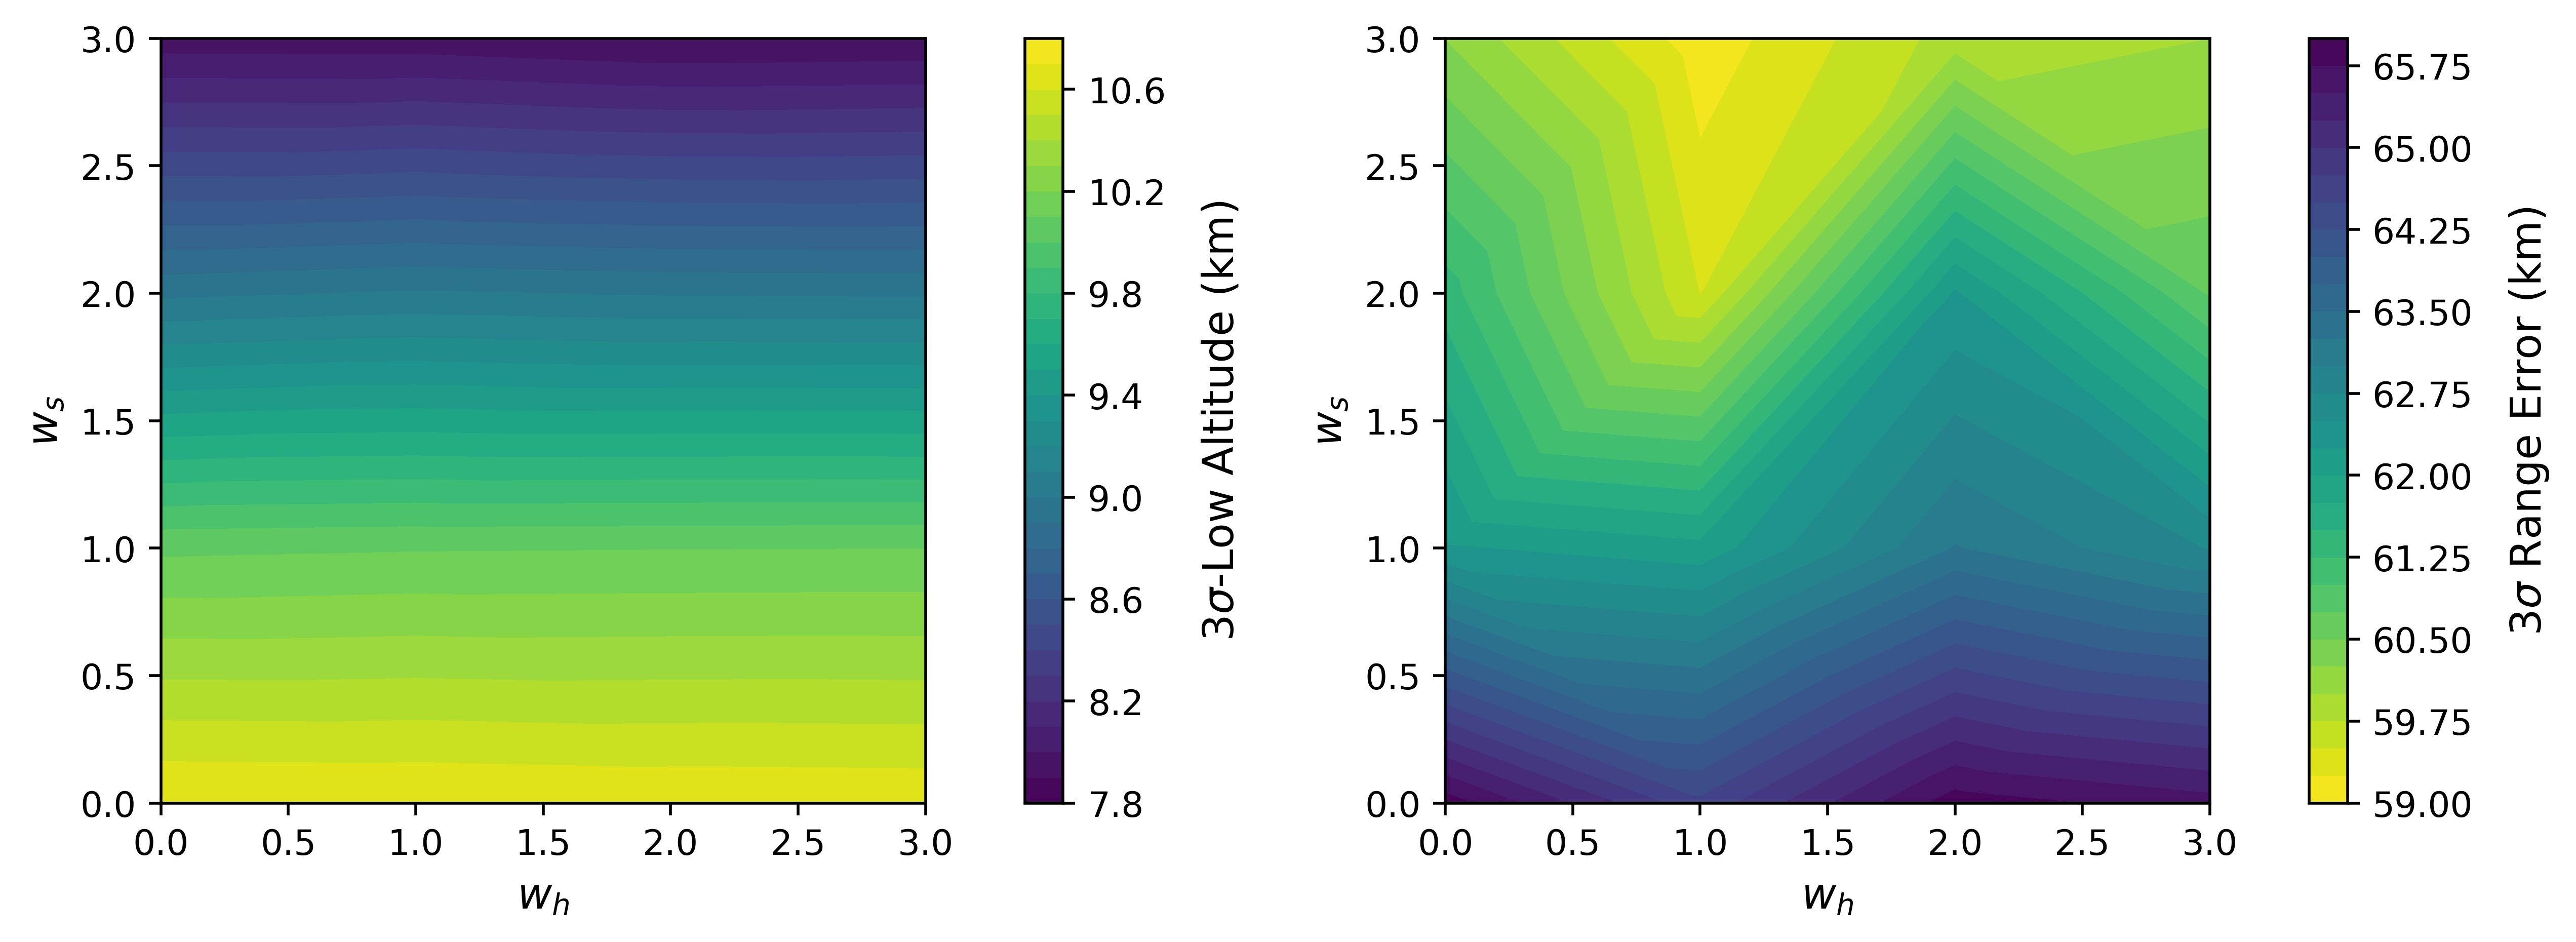
\includegraphics[width=1\textwidth]{Images/OpenLoop_WeightSweepMCResults}
	\caption{Monte Carlo statistics for the open-loop trajectory optimization. }
	\label{Fig:MCResultsOpenLoop}
\end{figure}
%\begin{figure}[h!]
%	\centering
%	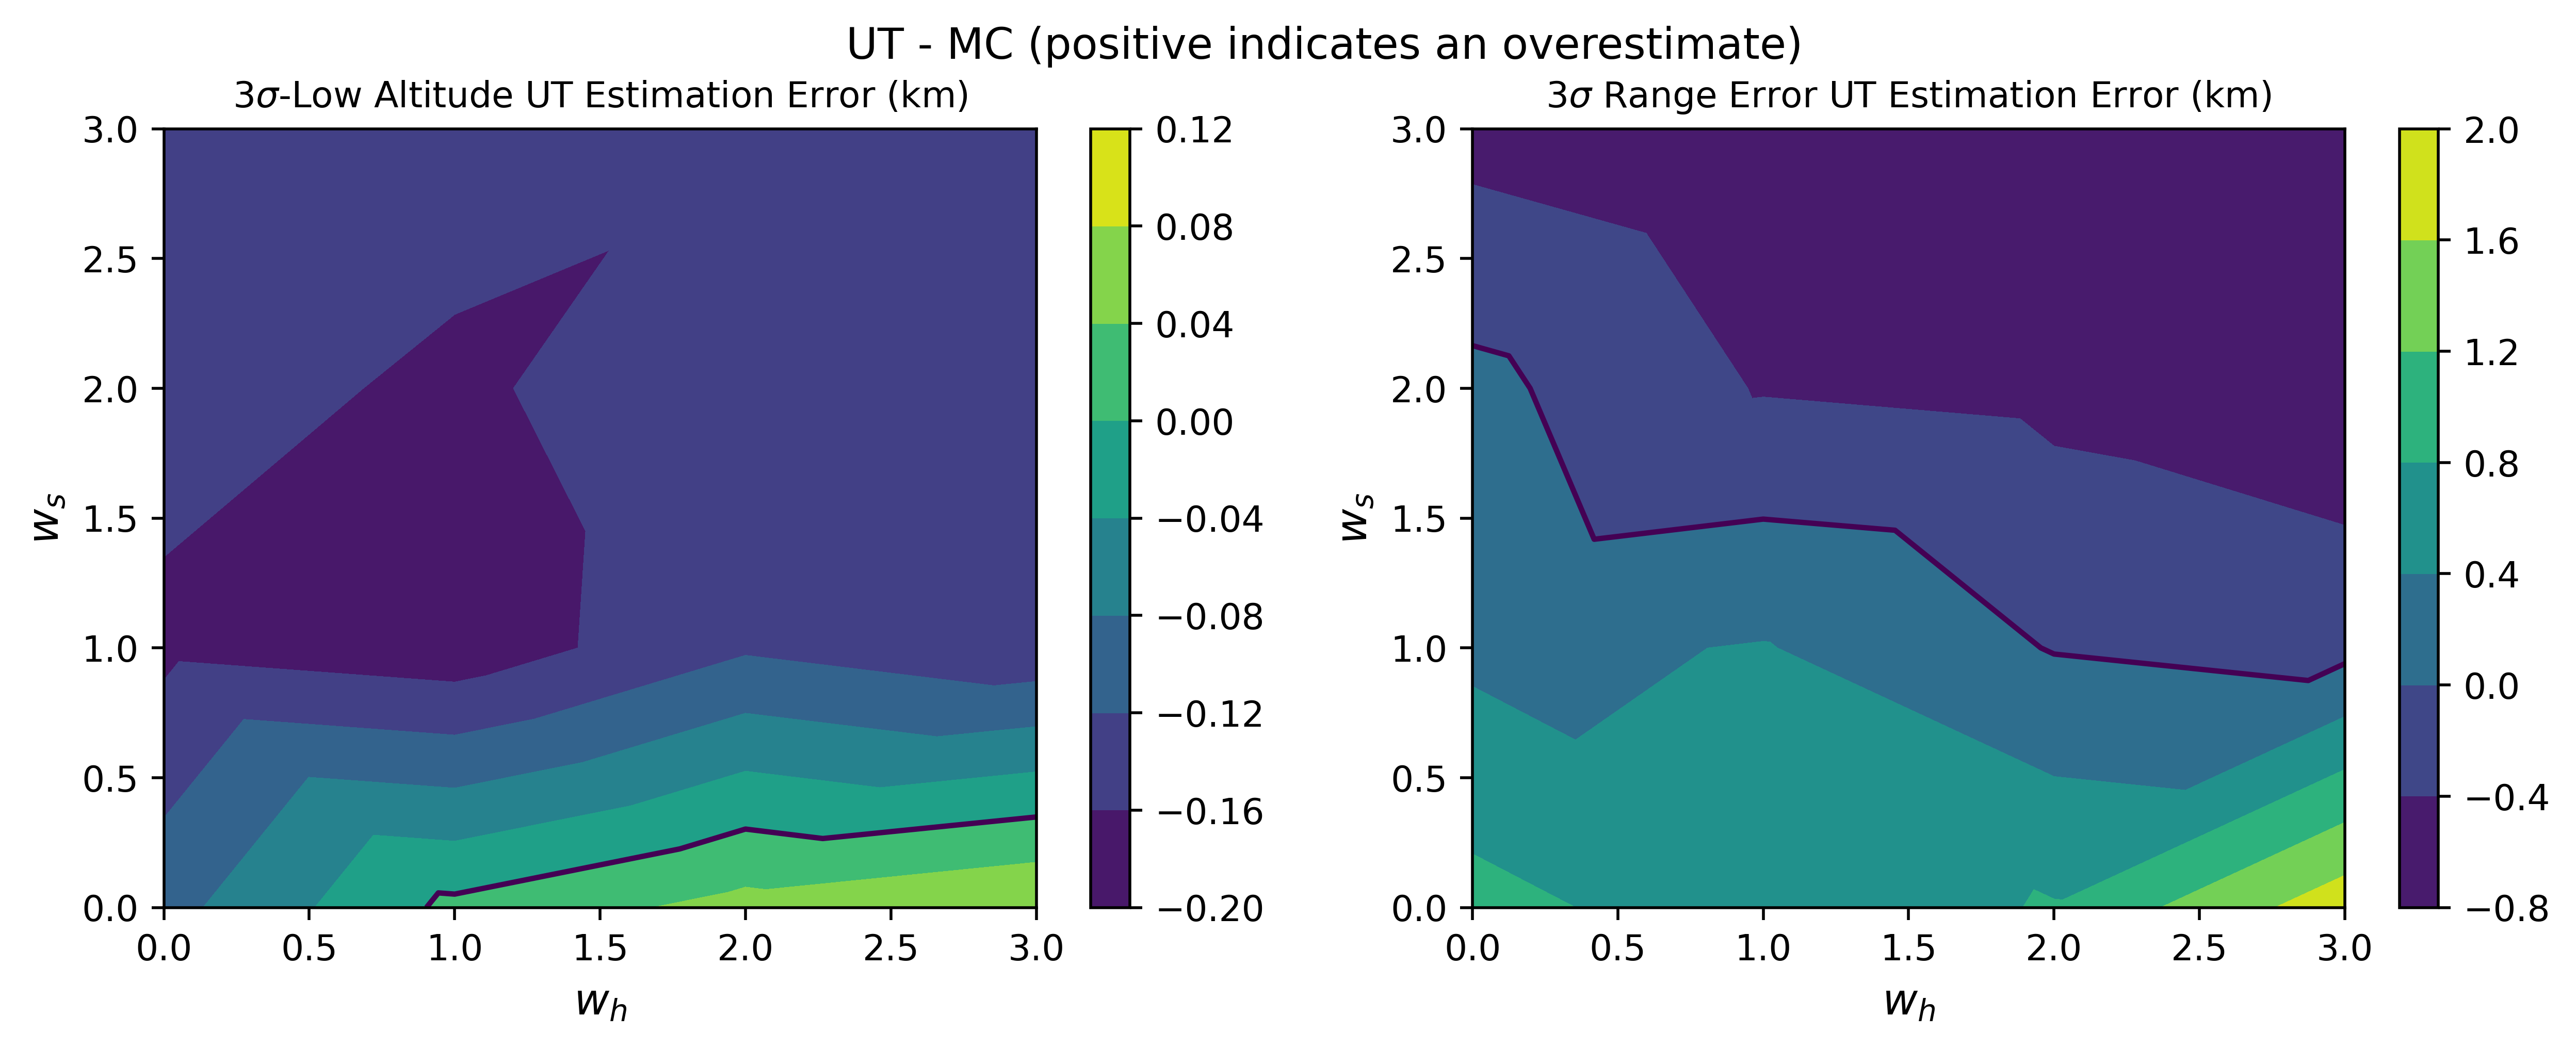
\includegraphics[width=1\textwidth]{Images/Reoptimized_WeightSweepError}
%	\caption{}
%	\label{Fig:MCErrorsOpenLoop}
%\end{figure}

\subsection{Closed-Loop Optimization}
%Maybe show ONLY  Monte Carlo results here. Then in the next section, do a detailed comparison. Justified by the fact that optimized gains are what we would want to use, so we should confirm those? But MC here already confirms. We could maybe get away with showing the UT only
Figure~\ref{Fig:MCResultsFixedGain} presents contours of the Monte Carlo estimated 3$\sigma$-low altitude and range errors for the closed-loop guidance with $K=K_2$. Introducing feedback allows the guidance to achieve 3$\sigma$ range errors as low as 5.6 km while also keeping the 3$\sigma$-low altitude above 9 km. This low altitude can be raised to 9.7 km at the expense of growing the 3$\sigma$ range errors to 14.6 km. The largest range errors occur when optimizing purely for mean altitude, $w_h=w_s=0$. 
\begin{figure}[h!]
	\centering
	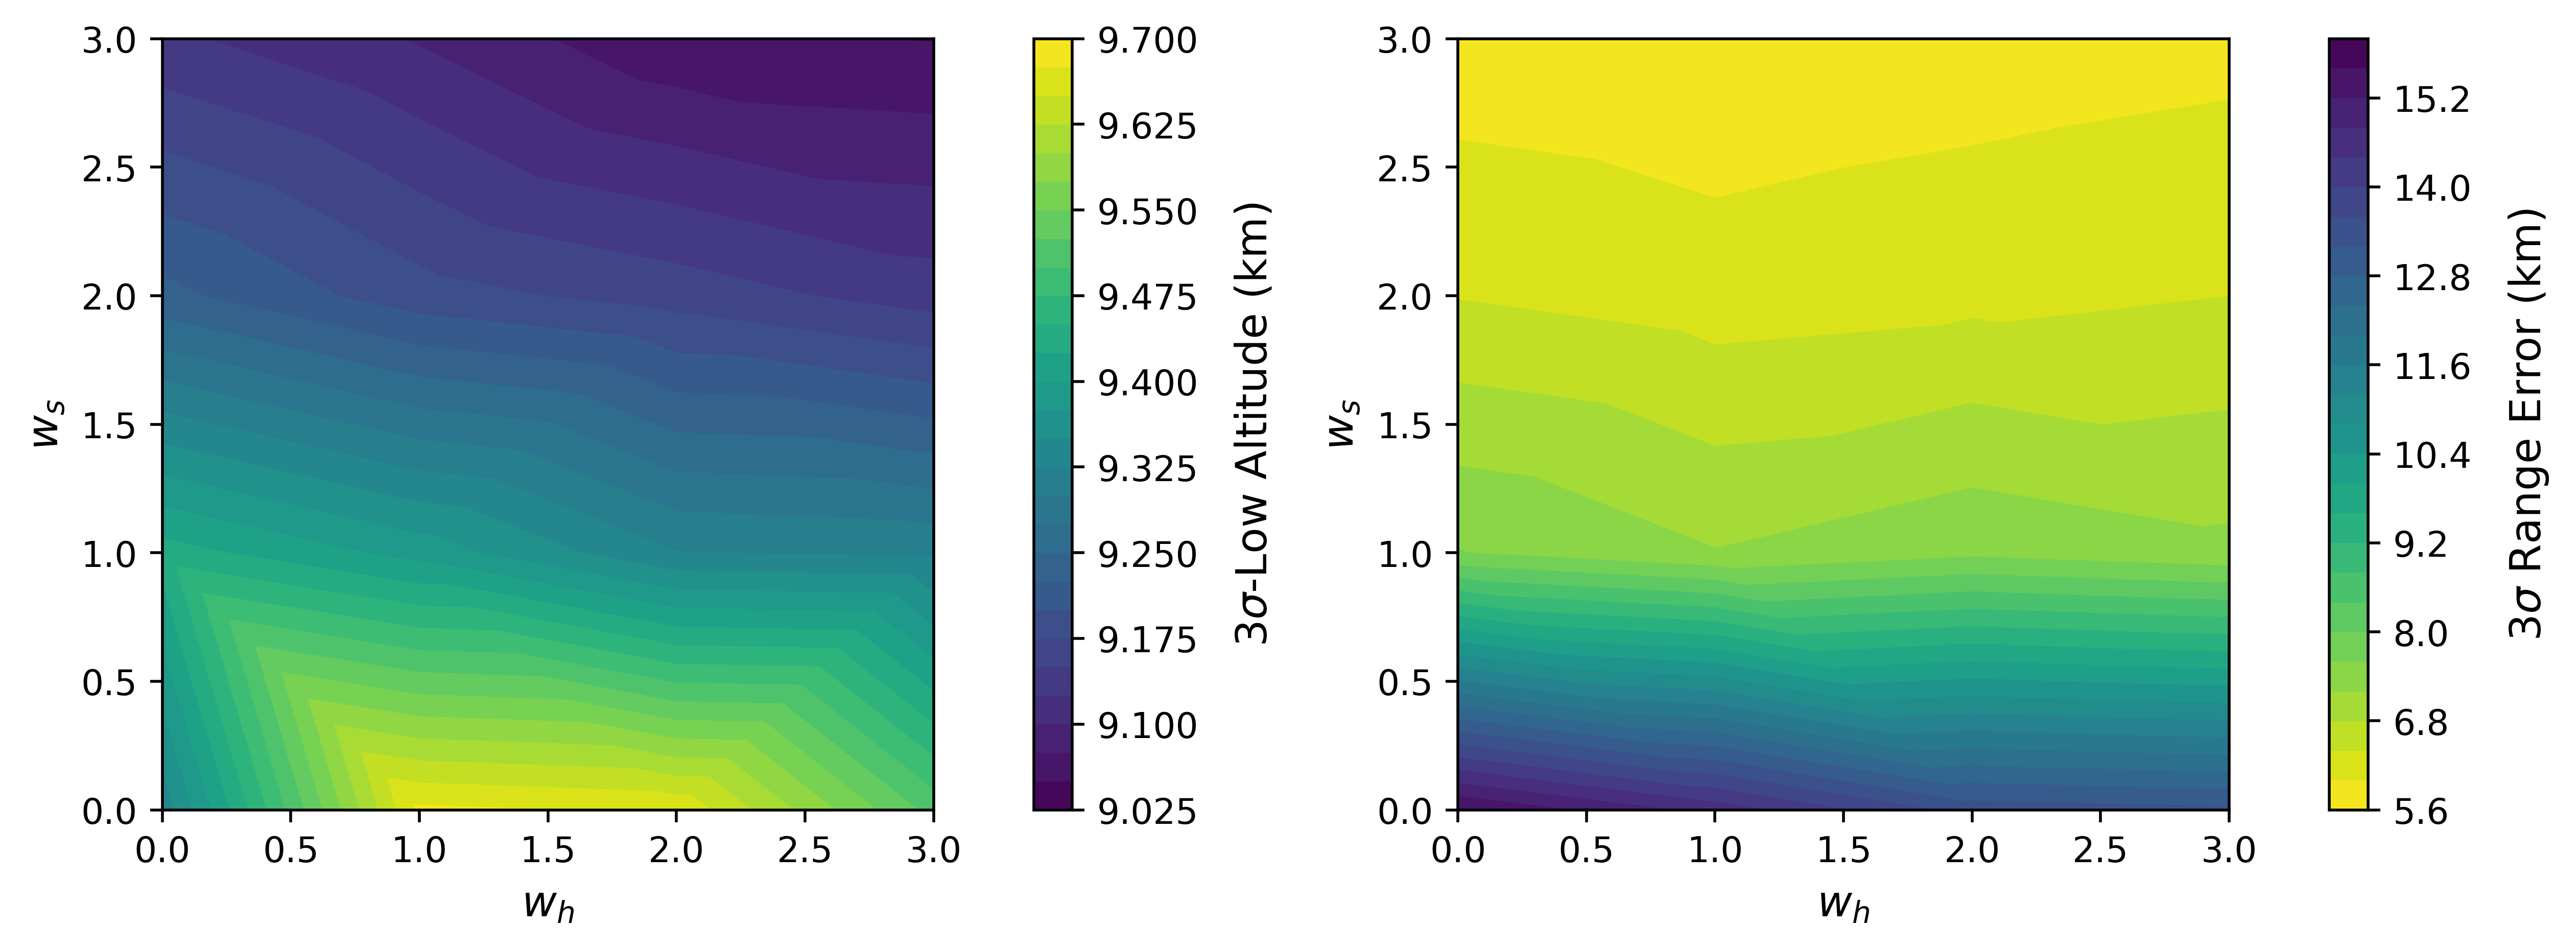
\includegraphics[width=1\textwidth]{Images/Reestimated_WeightSweepMCResults}
	\caption{Monte Carlo statistics for the closed-loop trajectory optimization with static gains.}
	\label{Fig:MCResultsFixedGain}
\end{figure}
Figure~\ref{Fig:MCErrorsFixedGain} shows the contours of the errors in the UT statistics compared to the Monte Carlo results. The error in 3$\sigma$-low altitude varies between a 120 m overestimate and a 360 underestimate. For a majority of $(w_h,w_s)$ pairs, the low altitude is underestimated. Although the estimation errors are generally small, they are large enough to affect the optimality of the solutions. The 3$\sigma$-low altitude should be maximized when $w_h=3$ and $w_s=0$, but instead the highest 3$\sigma$-low altitude is achieved for $w_h=1.5$. Notice that the suboptimality is also small, the solution for $w_h=3$ is only 150 m lower than for $w_h=1.5$. In contrast, the smallest range errors do occur for the $w_h=0,\,w_s=3$. 
\begin{figure}[h!]
	\centering
	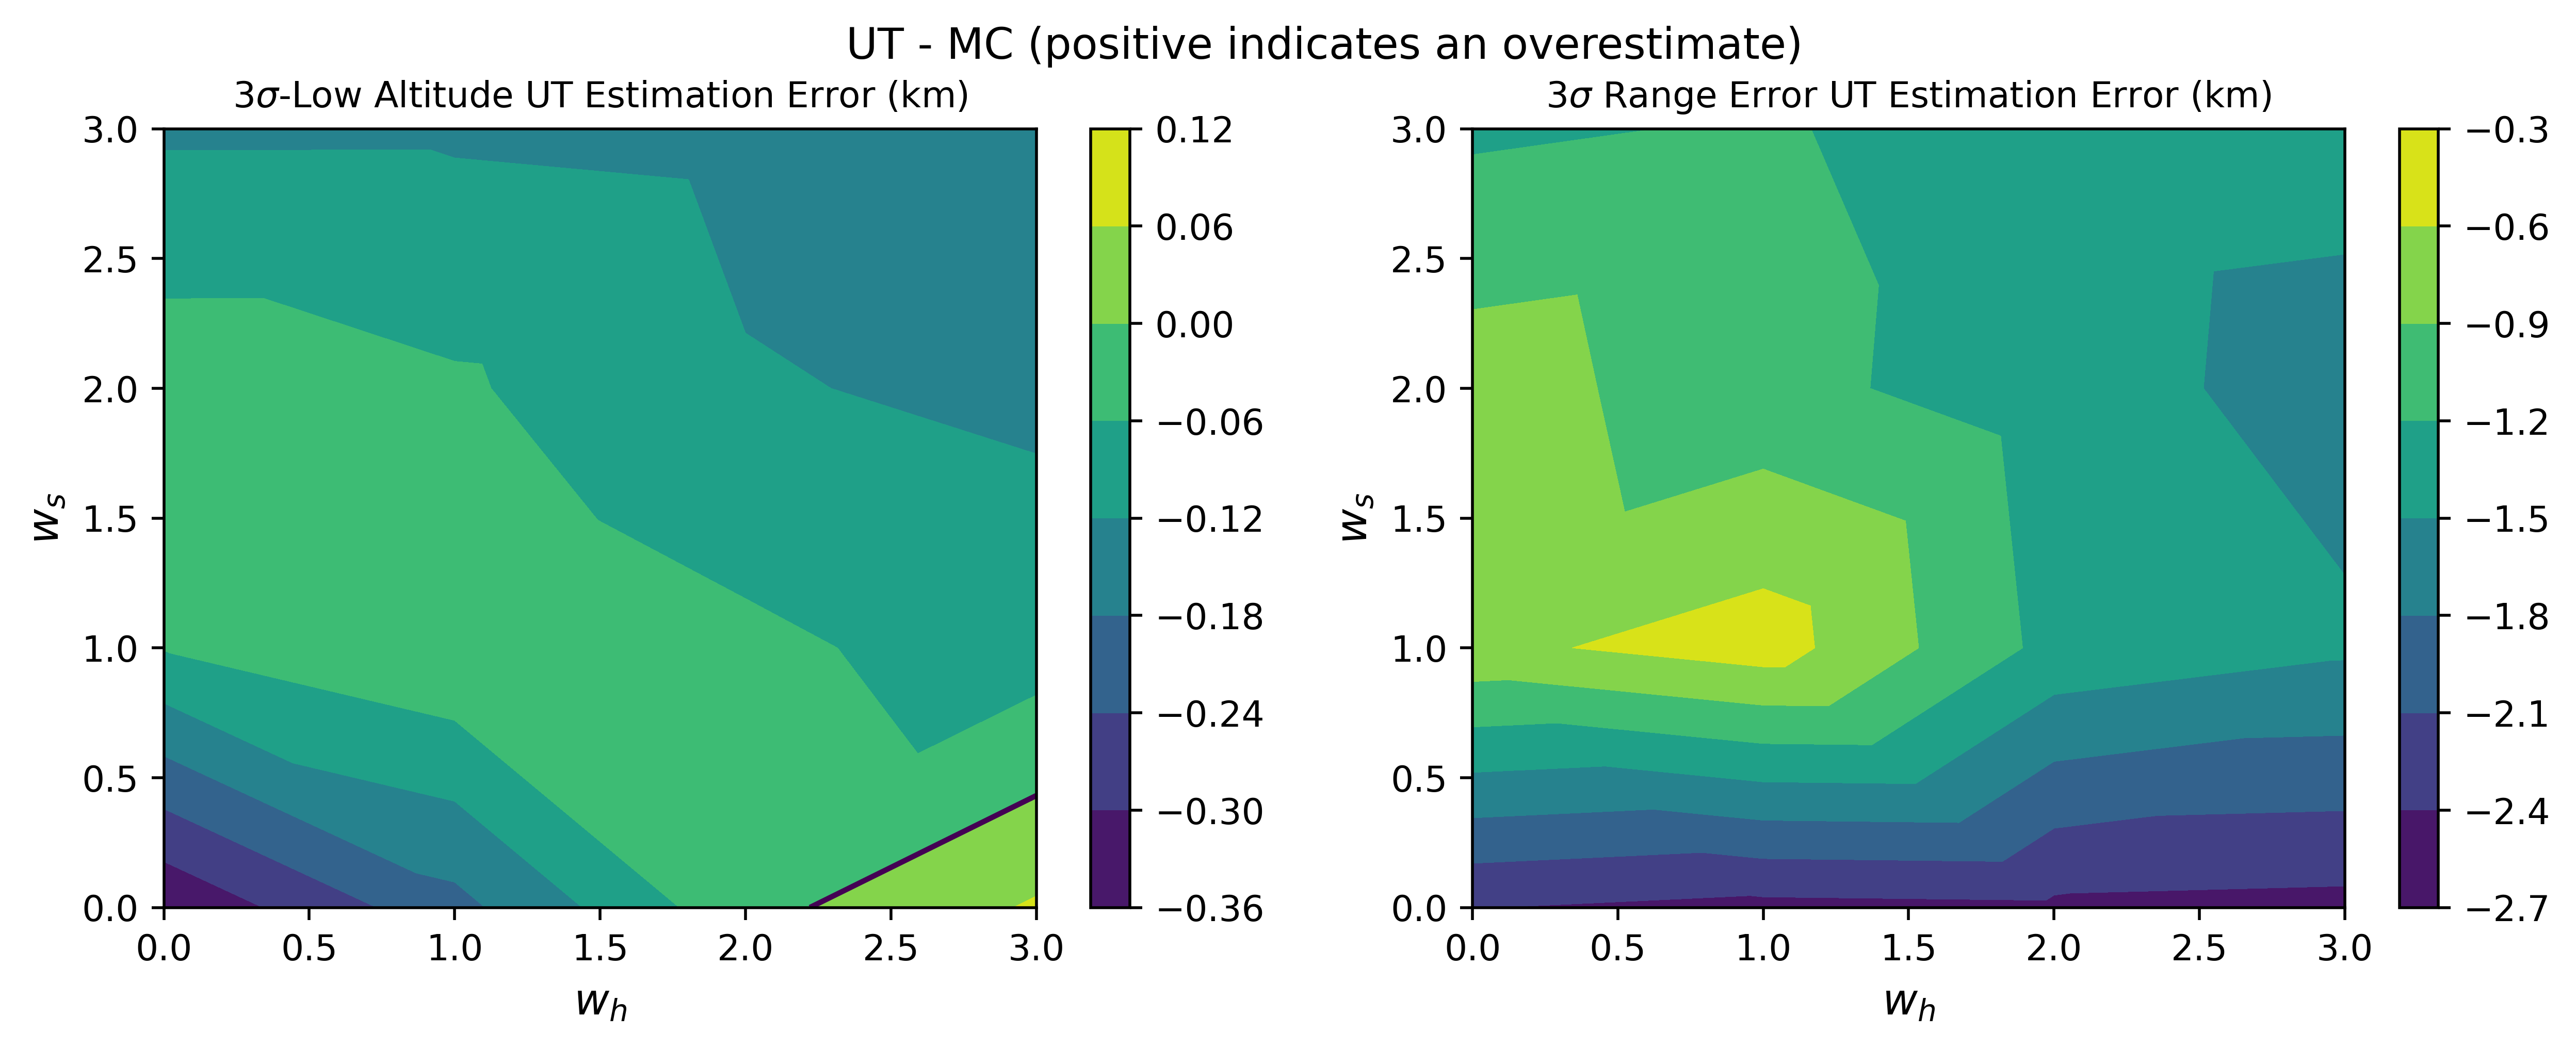
\includegraphics[width=1\textwidth]{Images/Reestimated_WeightSweepError}
	\caption{Unscented Transform estimation errors relative to Monte Carlo statistics for trajectory optimization with static feedback gains.}
	\label{Fig:MCErrorsFixedGain}
\end{figure}

\section{Joint Gain Optimization}
%Motivate the constant gain optimization here by showing an example of bad MC performance when simultaneously optimizing velocity-varying gains? Then show how well the constant gains can do when jointly optimized. 
In this section, the ROGP is again solved for a variety of weights but now the gains are treated as design parameters, and the DDP modification presented in Subsection~\ref{Sec:DesignOptimization} is used to jointly optimize them alongside the reference trajectory and control. As one might intuitively expect, the effect on the range of solutions is much more extreme with joint optimization than without. 

Figure~\ref{Fig:MCResultsOptGain} shows the contours. An additional 800 meters of low altitude can be gained (relative to the previous solutions with unoptimized gains), but at the expense of large $3\sigma$ range errors (above 40 km). However, a very tight range distribution of $3\sigma_s = 3$ km can be achieved while still maintaining a 9 km 3$\sigma$-low altitude for a variety of weights. The range error stops improving at approximately $w_s=1$, but the low altitude continues to decrease as $w_s$ is raised. Thus, an effective compromise might be $w_h=w_s=1$. 
%TODO: A Common trend among Figures~\ref{Fig:MCResultsOpenLoop},\ref{Fig:MCResultsFixedGain}, and \ref{Fig:MCResultsOptGain} is the relatively weak influence of $w_h$. While some weight prevents large altitude losses, even large weights cannot achieve more than a few hundred meters of improvement. 
\begin{figure}[h!]
	\centering
	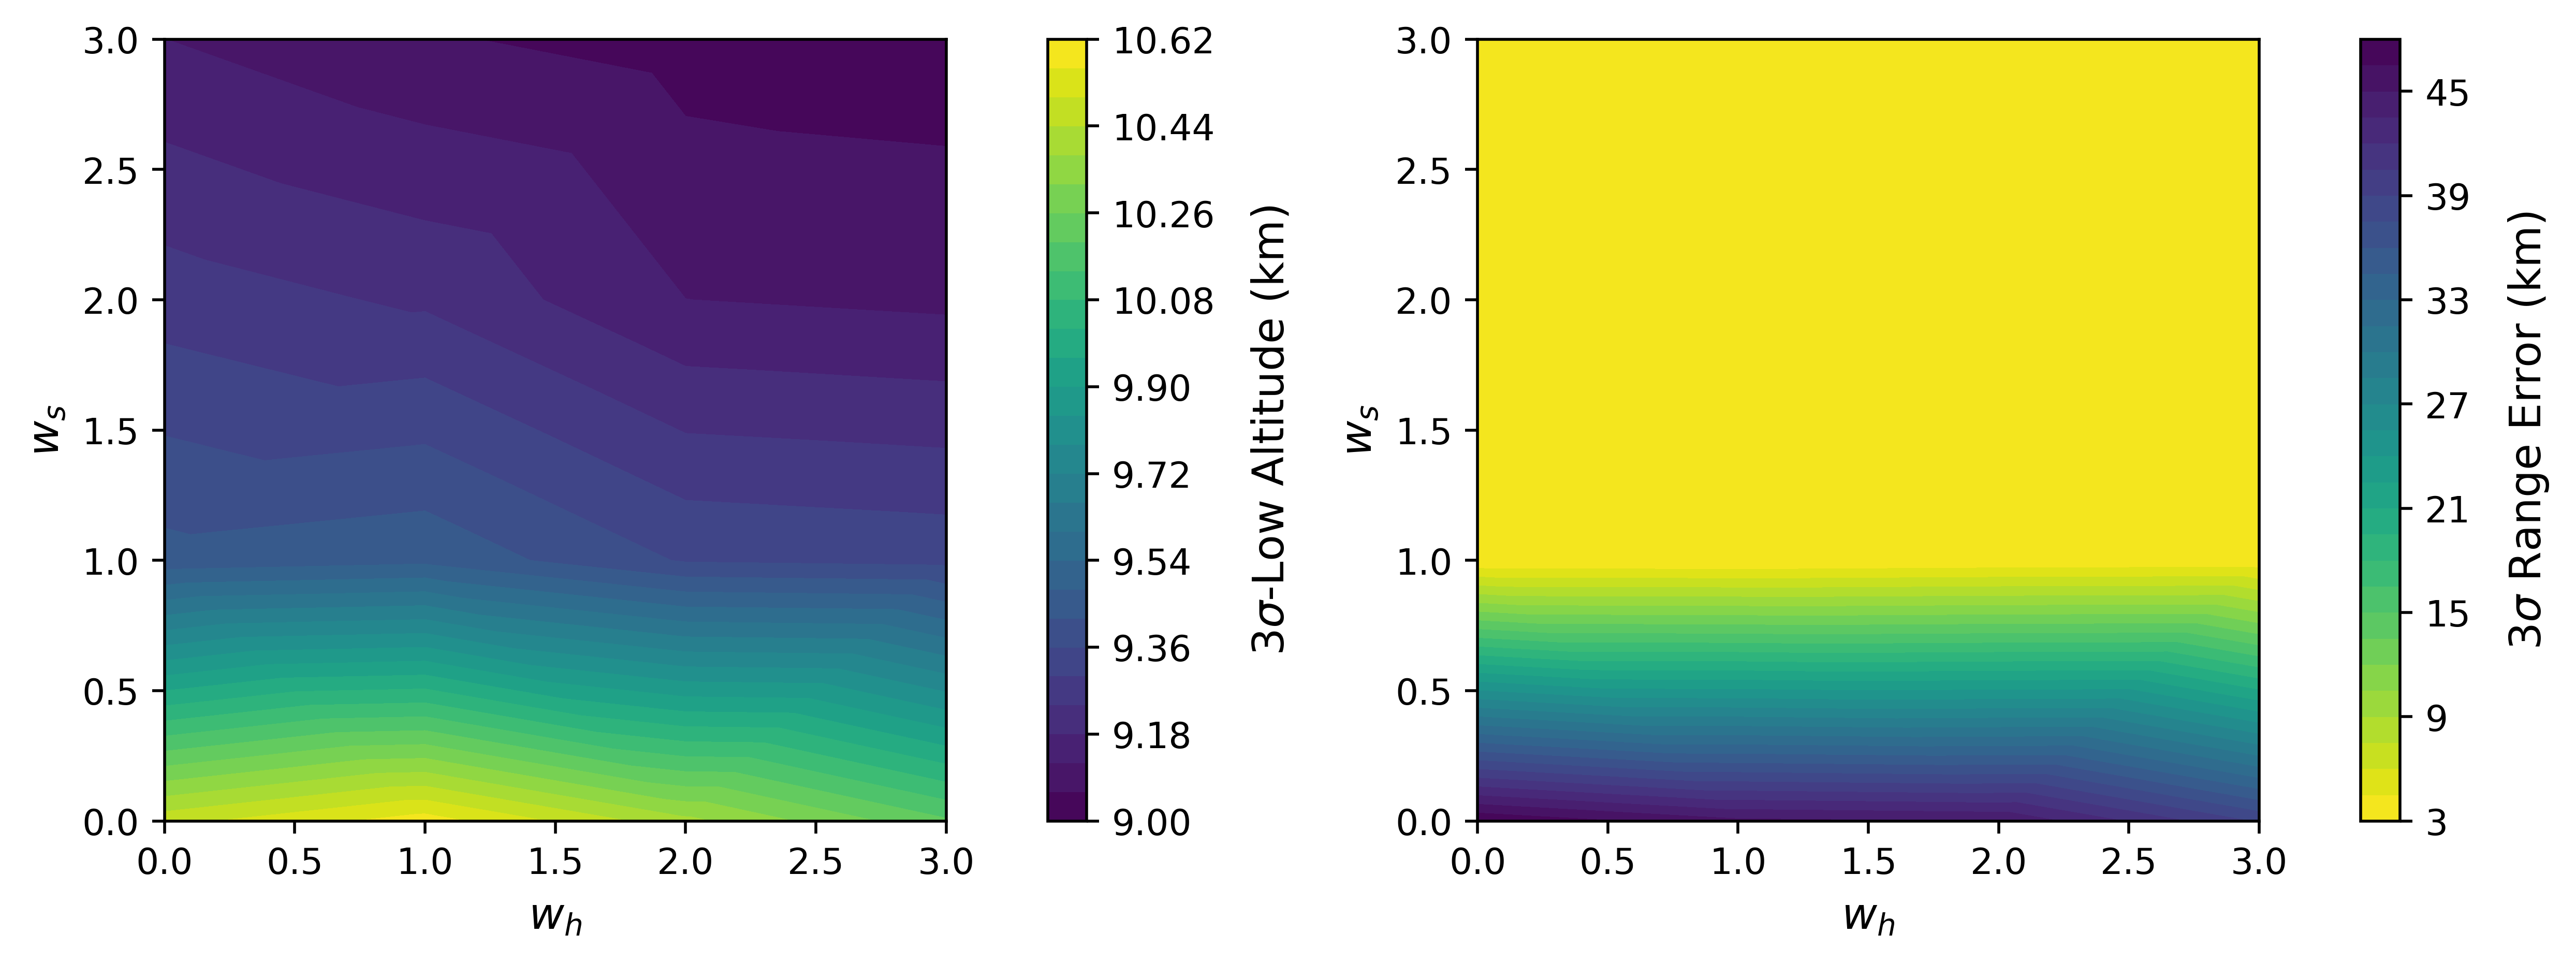
\includegraphics[width=1\textwidth]{Images/Reoptimized_WeightSweepMCResults}
	\caption{Monte Carlo statistics for jointly optimized static feedback gains.}
	\label{Fig:MCResultsOptGain}
\end{figure}
Figure~\ref{Fig:MCErrorsOptGain} shows the contours of the errors in the UT statistics compared to the Monte Carlo results. The dark line in each plot is the zero contour, where the UT and MC agree with approximately no error. Comparing Fig.~\ref{Fig:MCErrorsOptGain} to the previous error contour, Fig.~\ref{Fig:MCErrorsFixedGain}, we can see the effect to selecting the UT scaling parameter to minimize the estimation error in range error. For the fixed gain results in Fig.~\ref{Fig:MCErrorsFixedGain}, the range errors were uniformly underestimated, while for the optimized gains, the zero contour passes through $(w_h,w_s) = (1.5,1.5)$. 
The error in 3$\sigma$-low altitude varies between a 120 m overestimate and a 200 underestimate. Like the fixed gain results, the low altitude is underestimated for a majority of $(w_h,w_s)$ pairs. Estimation errors once again affect the optimality of the solutions. The highest 3$\sigma$-low altitude is achieved for $w_h=1$. 
\begin{figure}[h!]
	\centering
	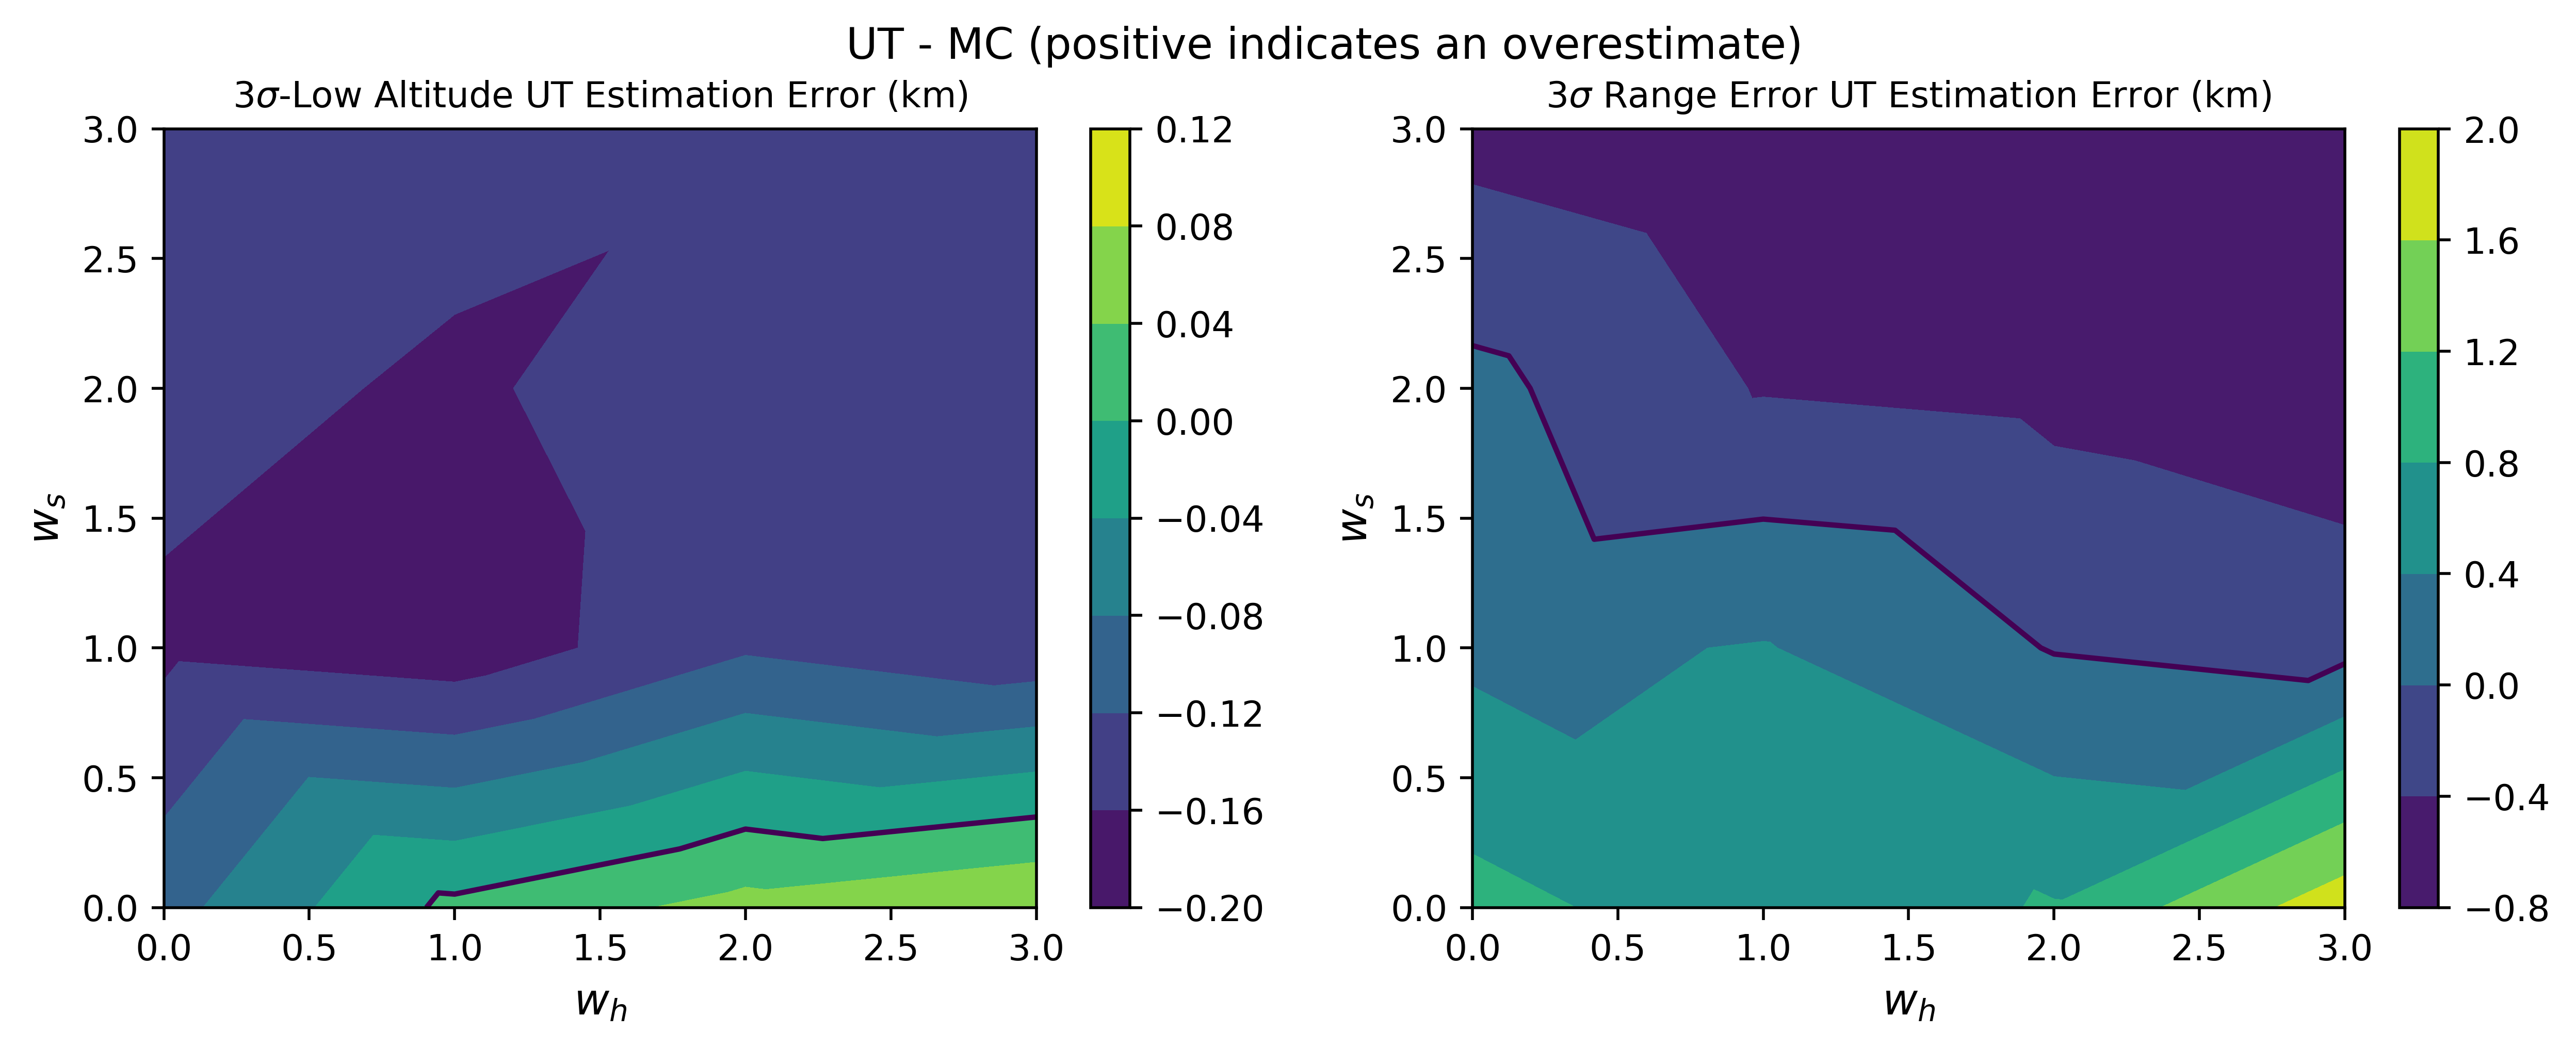
\includegraphics[width=1\textwidth]{Images/Reoptimized_WeightSweepError}
	\caption{Unscented Transform estimation errors relative to Monte Carlo statistics for jointly optimized static feedback gains.}
	\label{Fig:MCErrorsOptGain}
\end{figure}
Figure~\ref{Fig:MCTargetRange} depicts how the optimal downrange distance resulting from the solution to the ROGP varies with the weights. A very clear general trend is that more robust solutions, i.e., those with higher weight on either standard deviation, tend to target longer downrange distances. The total variation in target distance is about 30 km. The feedback gains have a large impact on these results. For comparison, Fig~\ref{Fig:MCTargetRangeOpenLoop} shows the target distances arising from the unguided open-loop optimization (corresponding to the contour in Fig.~\ref{Fig:MCResultsOpenLoop}). In the unguided case, there is virtually no change in target distance for different $w_h$, and the variation is exclusively with respect to $w_s$. The target distances are also noticeably shorter than in the guided case, roughly 40 km shorter on average.  
\begin{figure}[h!]
	\centering
	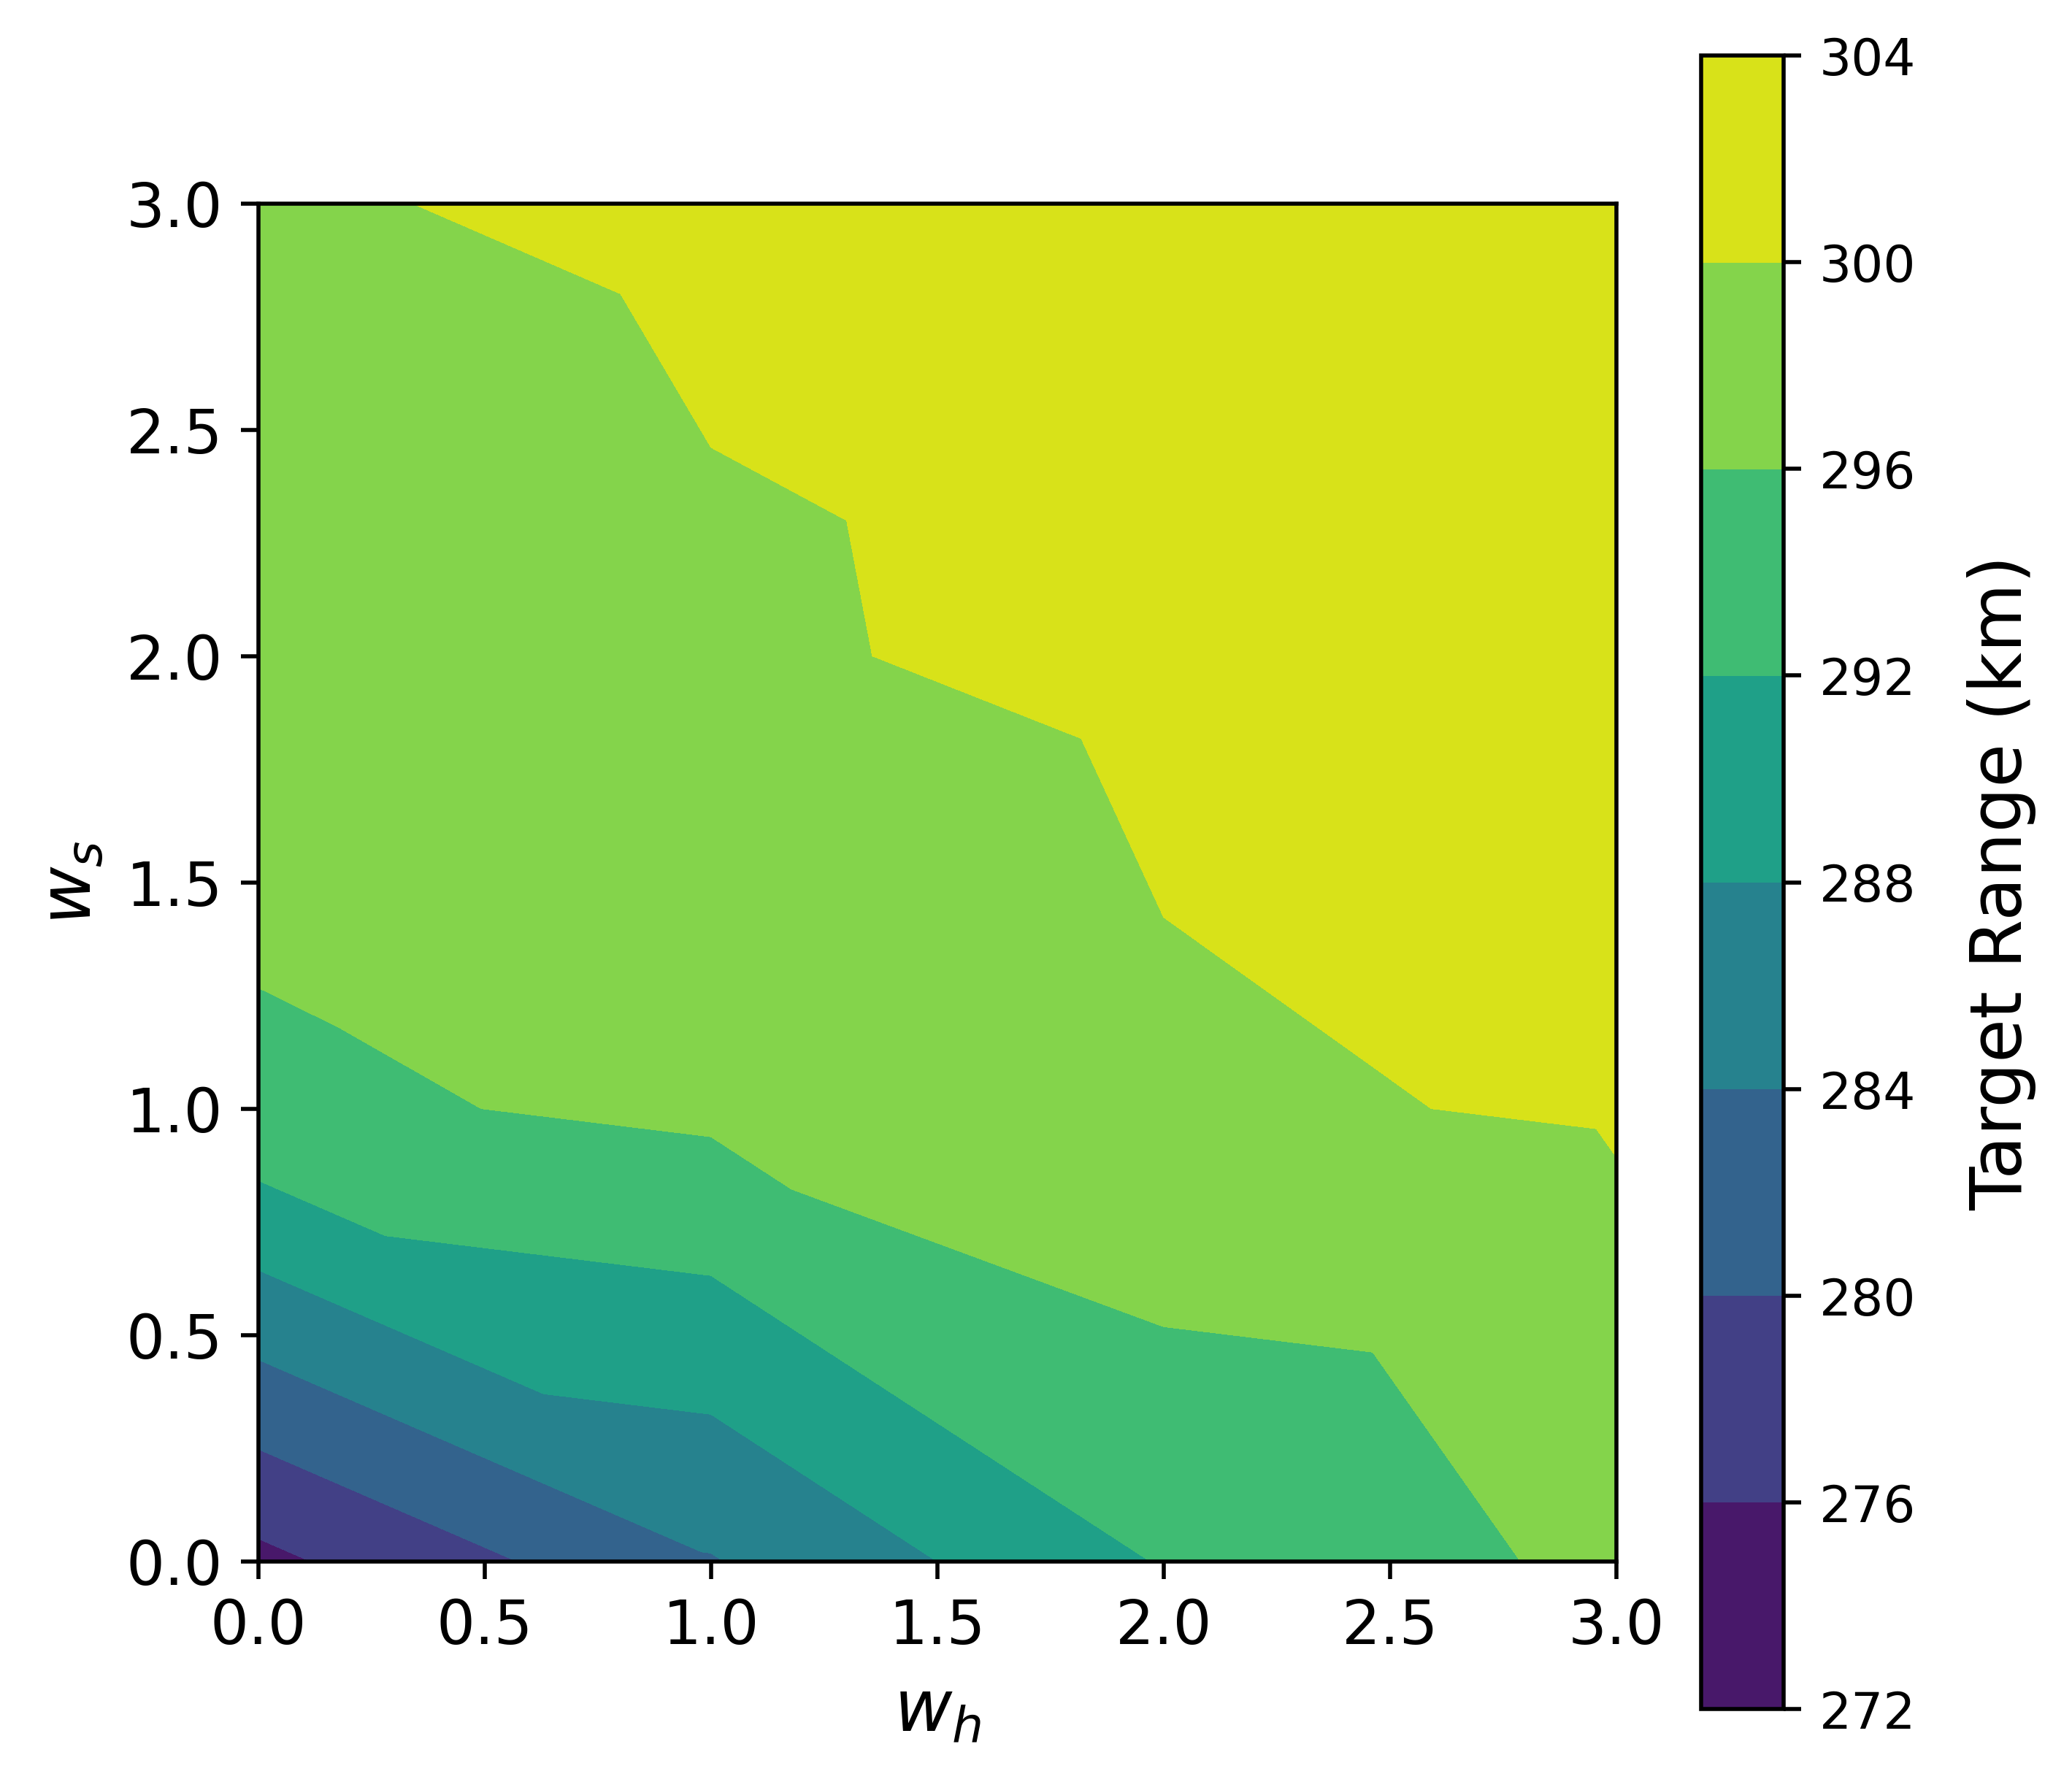
\includegraphics[width=1\textwidth]{Images/MSL_TargetRange}
	\caption{The optimal target range as a function of the performance weights.}
	\label{Fig:MCTargetRange}
\end{figure}
\begin{figure}[h!]
	\centering
	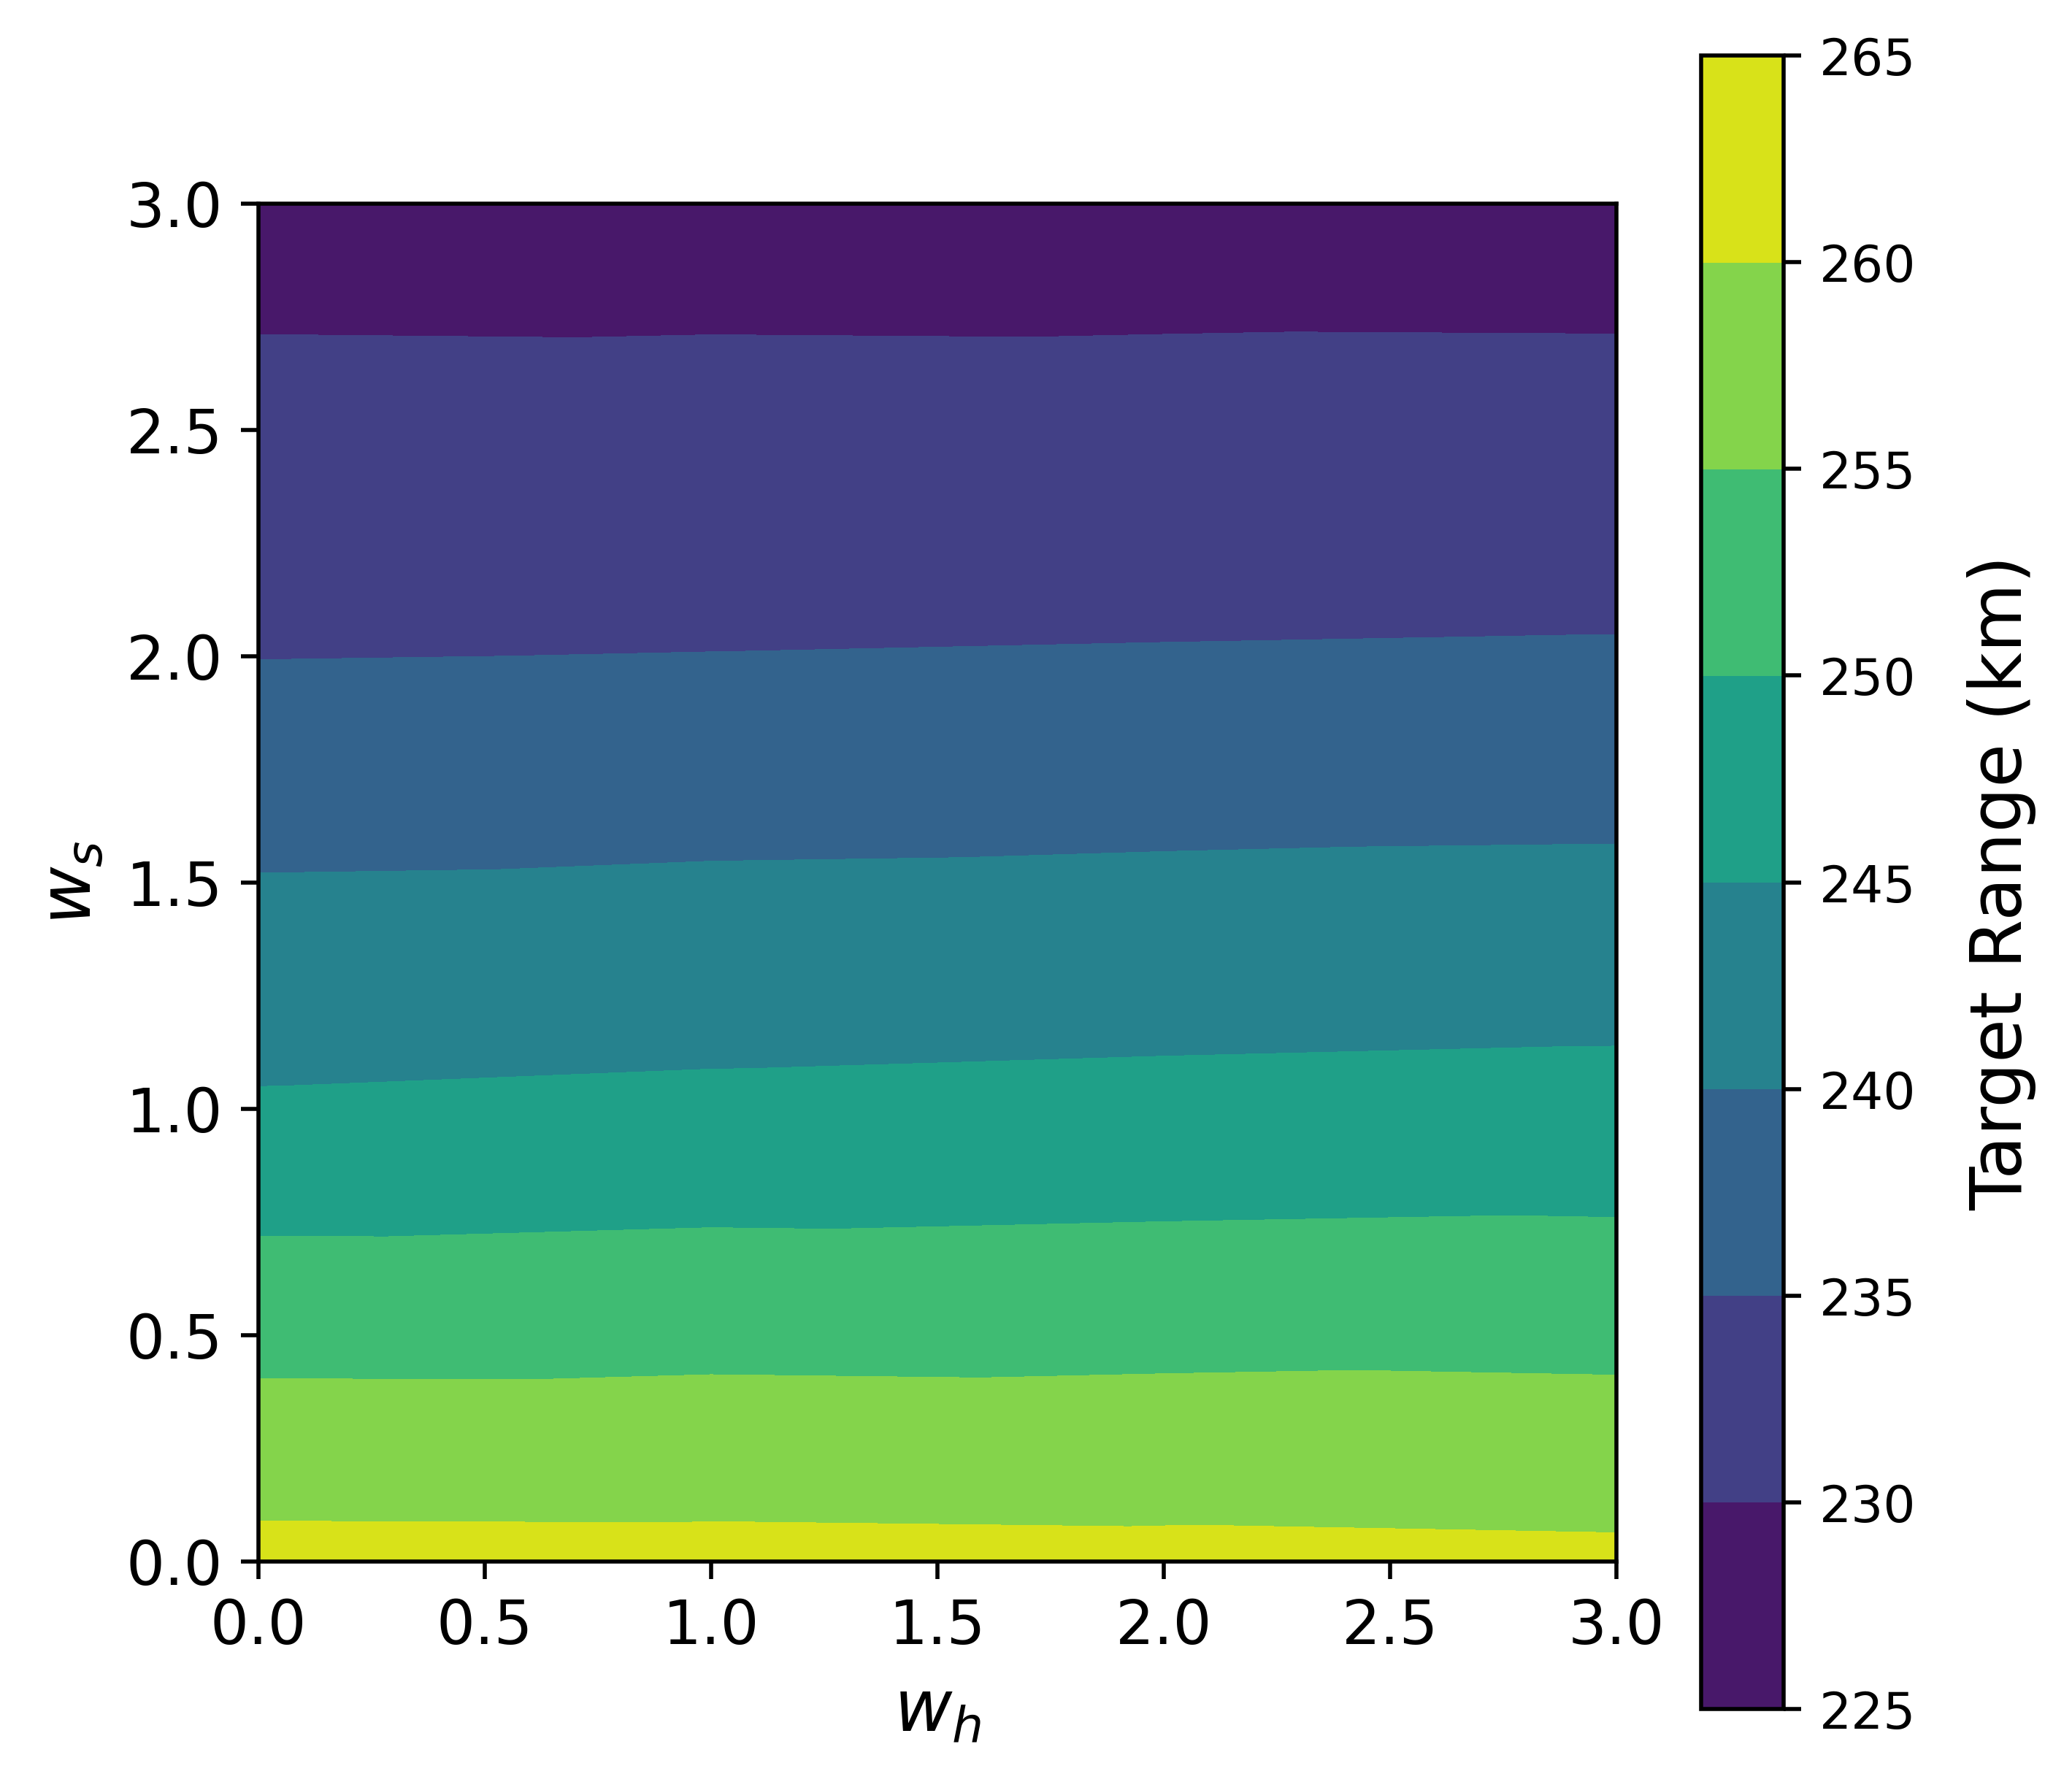
\includegraphics[width=1\textwidth]{Images/OpenLoop_TargetRange}
	\caption{The optimal target range as a function of the performance weights for an unguided vehicle.}
	\label{Fig:MCTargetRangeOpenLoop}
\end{figure}

\section{Detailed Comparison}
The previous sections considered the design space of the ROGP, examining the tradeoffs enabled by varying the weights in the performance index. In this section we present an in-depth look at a single solution, including visualizing the sample trajectories. We also perform further analysis to determine which uncertainties most strongly affect performance by applying the global sensitivity analysis technique known as Monte Carlo Filtering (MCF) \cite{MonteCarloFiltering}. We will examine the solution for $w_h=w_s=1$ with joint optimization of the feedback gains. 

The evolution of the marginal distribution of each state variable is shown in Fig.~\ref{Fig:DetailedTrajectory}, including 500 of the Monte Carlo sample trajectories, and the 3$\sigma$ bounds estimated via UT and MC. The UT bounds are nearly indistinguishable from the MC bounds. The $3\sigma$-low altitude is 9.5 km and the $3\sigma$ range error is 3.2 km. The lower right plot of Fig.~\ref{Fig:DetailedTrajectory} shows the reference control profile and 500 closed loop control profiles from the samples.
The reference control is saturated in the full lift up orientation for $v<1000$m/s. As noted in Ref.~\cite{MSL_EDL2}, such a maneuver results in higher deploy altitudes but also deteriorates the range performance as dispersed MC samples fall short of the target. However, the probabilistic nature of the performance index accounts for the expansion of the range errors when choosing the velocity at which to begin to command full lift up. In some sense, this result agrees with the MSL conclusion, which was that range control is less effective at velocities under 1100, and thus maintaining altitude by limiting the magnitude of the bank angle while also reducing cross range errors using heading alignment was an effective strategy to increase deploy altitudes without significantly compromising range accuracy. Here the robust optimal solution naturally leads to a similar approach by saturating the reference control, resulting in nearly all trajectories applying $u \ge 0.8$ for the remainder of entry. 
%This result is encouraging in the sense that commands during heading alignment would be similar in magnitude and thus potentially result in similar altitude and range performance despite using a different guidance.

Figure~\ref{Fig:DetailedScatter} shows a scatter plot of the terminal altitude and range, as well as 99\% confidence ellipses estimated via UT and MC. Here the UT estimation error is more clearly visible compared to the trajectory histories, but is small. Note also that while the UT has some estimation error in the covariance elements that results in a rotation of the confidence ellipse, these elements are not used in the problem formulation. The samples that terminated short of the target (positive range error) demonstrate the earlier point about the ``brittleness" of solutions that do not leave margin at low velocities. However, we remark that this is remedied by applying a larger weight on $\sigma_s$, which will naturally result in less saturation. 
\begin{figure}[h!]
	\centering
	\includegraphics[width=1\textwidth]{Images/Trajectory/MCGridExample}
	\caption{Sample trajectories and 3$\sigma$ bounds estimated by MC and UT.}
	\label{Fig:DetailedTrajectory}
\end{figure}
\begin{figure}[h!]
	\centering
	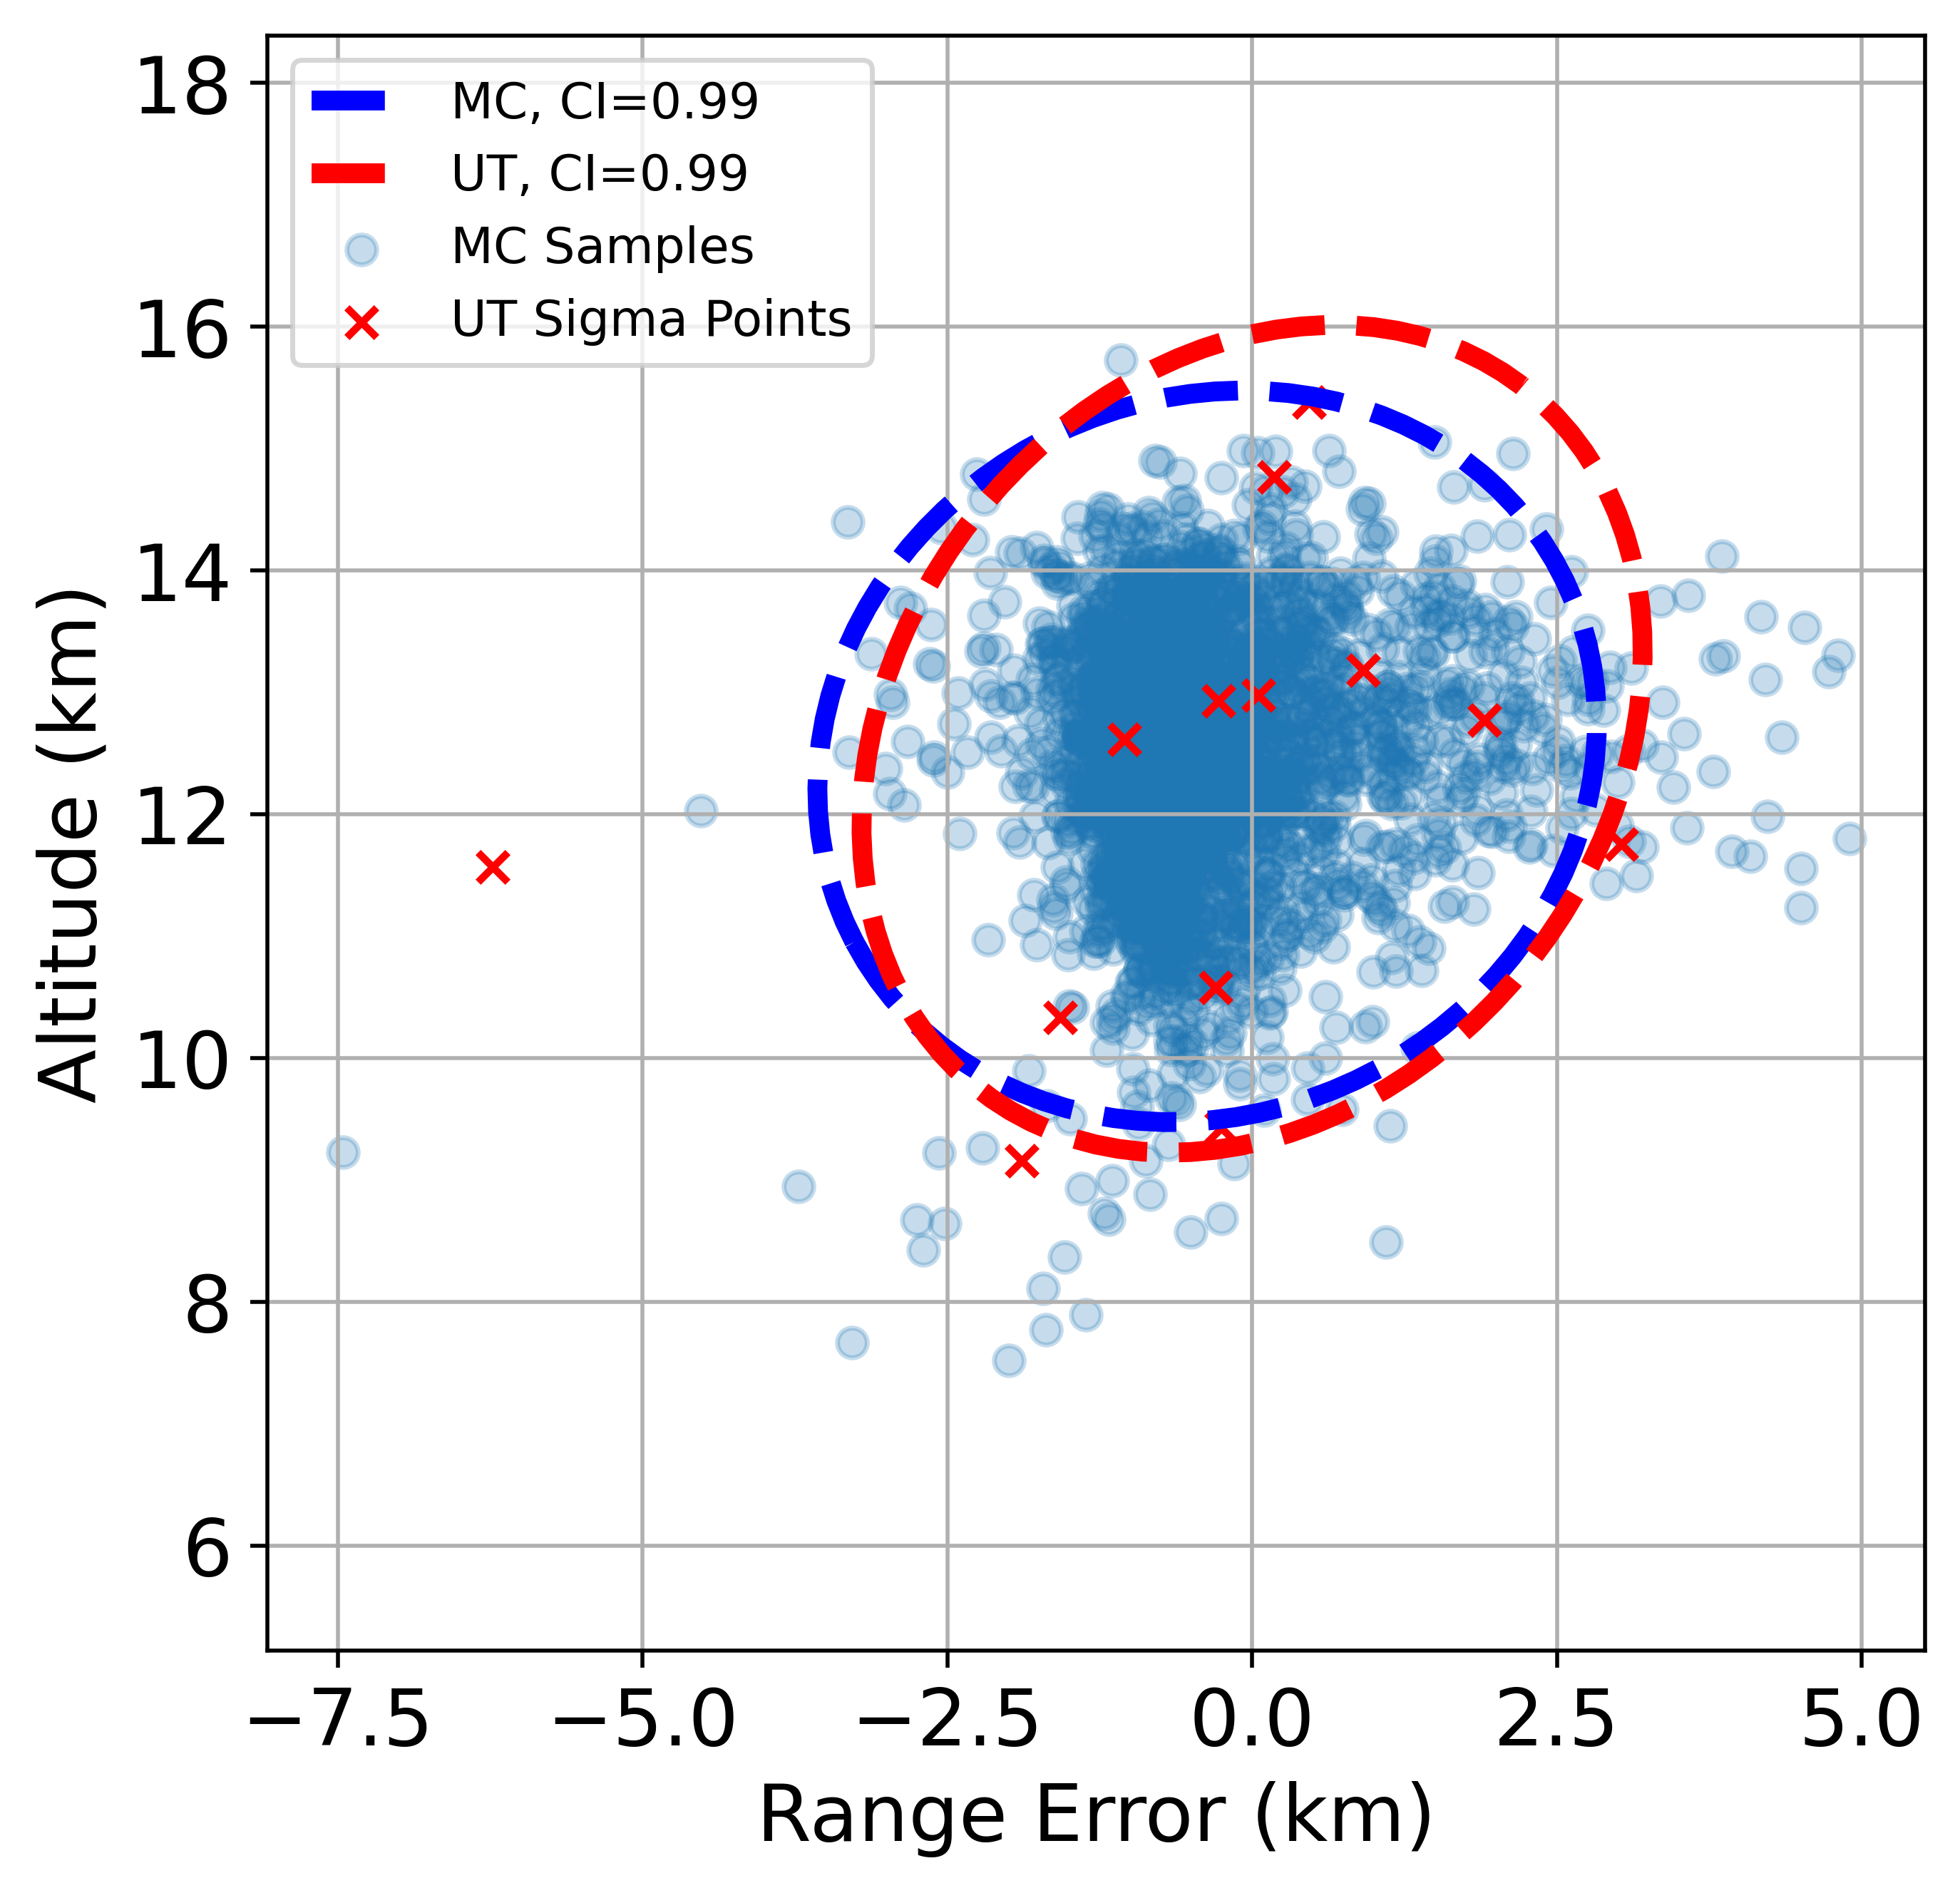
\includegraphics[width=1\textwidth]{Images/Trajectory/AltitudeRangeScatterExample}
	\caption{Terminal altitude and range performance.}
	\label{Fig:DetailedScatter}
\end{figure}
%TODO: Needs more complete discussion, the numbers aren't there
%TODO: Talk about the control saturation at the end, fragility, ability to plan for large Covariance if that's the important metric or pass/fail. 
\subsection{Sensitivity Analysis}
The numerical results show a clear tradeoff between terminal altitude and range performance. In this section we utilize MCF to determine which uncertainties are the dominant source of low altitude or high range error. MCF is a density-based, global sensitivity analysis method compatible with MC data. 

Density-based sensitivity analysis considers the PDF or CDF of an output variable, in contrast to variance-based methods that consider the second moment of the output. 
In the context of sensitivity analysis, global means to consider input variations in the entire feasible space, in contrast to local methods, like partial derivatives, that are evaluated at a single point. 

MCF proceeds as follows: given an output variable of interest, $y$, divide the MC samples into two groups based on a selected criteria. For each input variable, $x_i$, compute the ECDF of each group. Next, the the two-sample Kolmogorov–Smirnov statistic, a measure of the distance between two ECDFs, is computed as
 \begin{align}
	KS = \max_{x_i} | F_1(x_i) - F_2(x_i) | \label{Eq:KSTest}
\end{align}
where $F_i$ is the ECDF of the $i^{\mathrm{th}}$ input. Notice the the KS test is sensitive to both the shape and location of the CDF. Finally, the inputs are ranked according to their KS statistic. In our application the outputs are terminal altitude and range. For altitude, the criteria is that the sample altitude is less than the mean altitude of the samples. For range, the criteria is that the absolute error is greater than the mean absolute error. Note that the two groups do not (and need not) contain the same number of samples. Performing this test for the two different outputs and criteria are summarized in Table~\ref{Table:MCF}. The dominant sources of lower than average altitude are density and ballistic coefficient, and to a lesser extent initial errors in range and altitude. The entry flight path angle has a limited effect. Conversely, the initial state errors in altitude, range and significantly impact the guidance performance. The flight path angle and lift-to-drag ratio have a lesser effect on the range errors, and density and ballistic have little to no impact. From these results, it is clear that the uncertainties affect our quantities of interest in different ways; the only uncertainty in the top 3 of both outputs is the initial altitude. One conclusion is that in order to simultaneously achieve high altitude and low range error is to effectively mitigate all of the different sources of uncertainty. 
%TODO: Compare to MSL - I think they largely found the same thing 
% Direct quotes that should be reword:
%Density-based sensitivity indices are moment-independent indices because, by definition, they consider the entire probability distribution of the output rather than one of its moments only.
\begin{table}[h!]
	\centering
	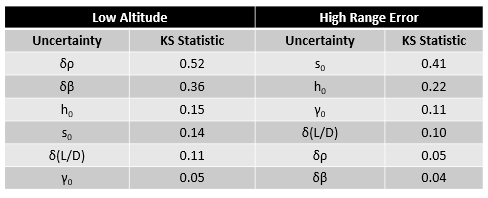
\includegraphics[width=1\textwidth]{Images/MCFTable}
	\caption{KS statistics estimating the sensitivity of terminal altitude and range to the uncertain input variables.}
	\label{Table:MCF}
\end{table}

\section{Convergence Properties}\label{Sec:ConvergenceProperties}
In this section we examine the convergence of solutions using 1) the full DDP algorithm, 2) DDP with the $\mathbf{f}_{\state\state}=\zero,\, \mathbf{f}_{\control\state}=\zero$ modification proposed in Subsection~\ref{Sec:DDP_Simplification} (labeled DDP-ControlHessian in figures), and the iterated Linear Quadratic Regulator~\cite{iLQG} (iLQR) variation where additionally $\mathbf{f}_{\control\control}=\zero$. We solve the ROGP for $w_h=w_s=1$ with each method. The primary metrics that we are interested in are the total cost, the total number of iterations, the time spent computing derivatives, and the maximum of the norm of the gradient of the value function with respect to the controls over the entire trajectory. We will also examine the linesearch stepsizes. In this example, only the parametric uncertainties in ($[L/D,\beta,\rho]$) are considered; the initial state uncertainty is set to zero. The reason is that the number of sigma points, and thus the number of states in the extended state vector, depends on the uncertainty dimension. While there is no difficulty in solving the full six dimensional problem (and indeed larger sizes) using iLQR or DDP-ControlHessian, the laptop used to solve the ROGP could not even store the full Hessian matrices for all $N=250$ steps used in the original DDP formulation.
\begin{figure}[h!]
	\centering
	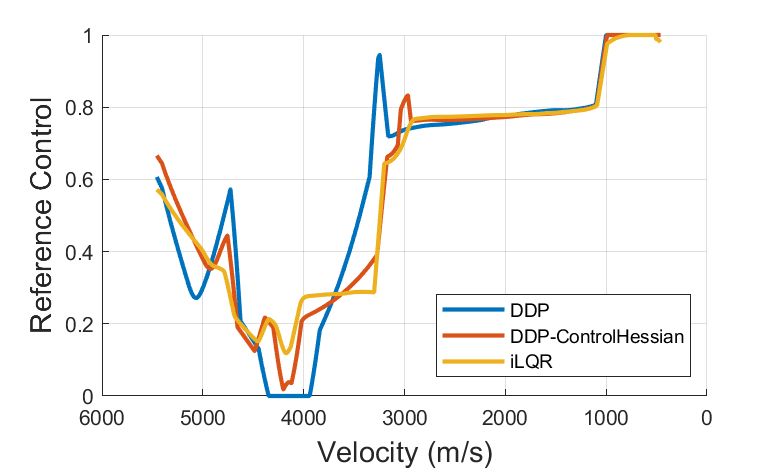
\includegraphics[width=0.75\textwidth]{Images/Convergence/ControlProfiles}
	\caption{Total cost per iteration}
	\label{Fig:ConvergeControls}
\end{figure}
\begin{figure}[h!]
	\centering
	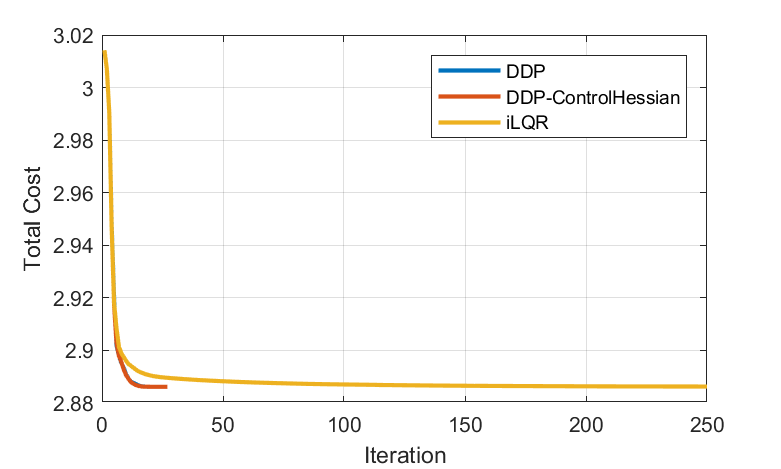
\includegraphics[width=0.75\textwidth]{Images/Convergence/cost}
	\caption{Total cost per iteration}
	\label{Fig:ConvergeCost}
\end{figure}
\begin{figure}[h!]
	\centering
	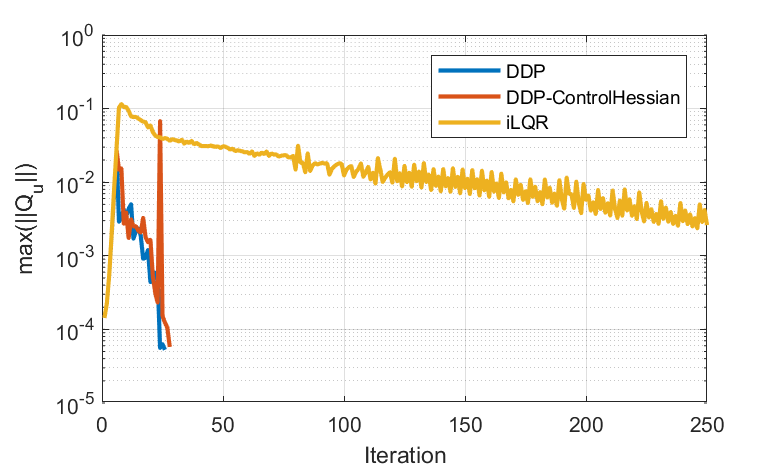
\includegraphics[width=0.75\textwidth]{Images/Convergence/grad_norm}
	\caption{Maximum control gradient norm over all timesteps.}
	\label{Fig:ConvergeGradient}
\end{figure}
\begin{figure}[h!]
	\centering
	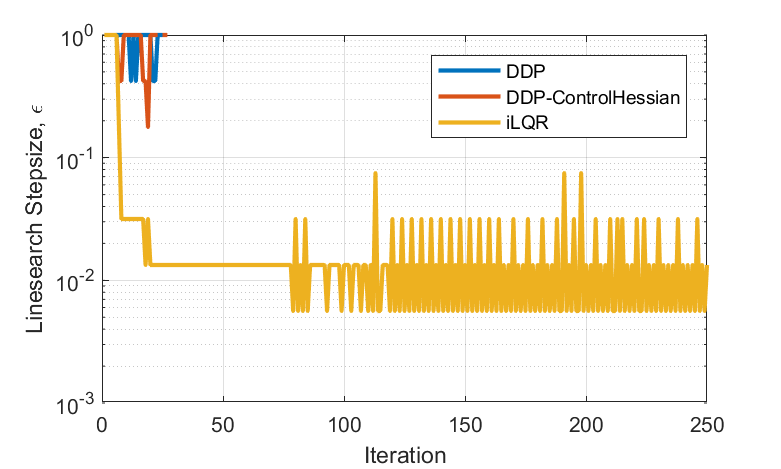
\includegraphics[width=0.75\textwidth]{Images/Convergence/alpha}
	\caption{Backtracking linesearch stepsize per iteration.}
	\label{Fig:ConvergeStepsize}
\end{figure}
\begin{figure}[h!]
	\centering
	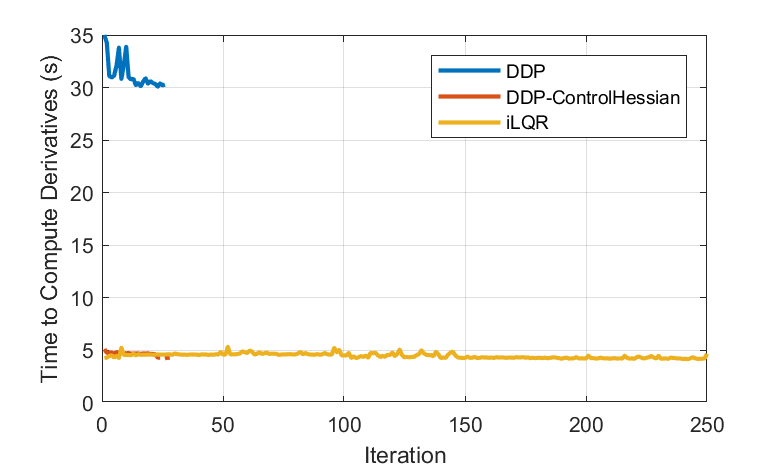
\includegraphics[width=0.75\textwidth]{Images/Convergence/time_derivs}
	\caption{Time in seconds spent computing derivatives of the cost and dynamics at each iteration.}
	\label{Fig:ConvergeTime}
\end{figure}


Figure~\ref{Fig:ConvergeControls} shows the resulting reference controls. While the results are similar, the three methods do not converge to identical solutions. 
Figure~\ref{Fig:ConvergeStepsize} shows the total cost at each iteration. Full DDP achieves the lowest cost of 2.868 after 81 iterations. Control Hessian-only DDP achieves a cost of 2.870 after 46 iterations, and iLQR has the highest cost, 2.871, and still has not terminated after 250 iterations. Figure~\ref{Fig:ConvergeGradient} shows the maximum gradient at each iteration. Unlike the DDP variants, the gradient never meets the exit criteria and thus is terminated based on the number of iterations. 
Figure~\ref{Fig:ConvergeStepsize} shows the stepsizes accepted in the linesearch procedure. Both DDP variants frequently accepted the full step $\epsilon=1$, while iLQR always took considerably smaller steps on the order of $ 10^{-2} $. Finally, Fig.~\ref{Fig:ConvergeTime} shows the drastic, nearly 10x reduction in time spent computing the derivatives resulting from omitting Hessian terms. The average times were $47.7$ s, 5.6 s, and 5.2 s, respectively. 
This example shows that, for this problem, retaining the second order derivatives with respect to the controls achieves nearly the same convergence as the full DDP algorithm while being only mildly more expensive to compute than the iLQR solution. 

We also considered different initial guesses at the optimal control to determine if the solution is sensitive to the initialization. In contrast to the linear ramp up guess, we considered a linear ramp down from 1 to 0, as well as two constant guess of full lift up, $u_{\mathrm{ref}}=1$ and half lift up $u_{\mathrm{ref}}=0.5$. Only the control hessian is retained, and the final cost and total iterations are summarized in Table~\ref{Table:ConvergeGuesses}. All four solutions converge to nearly identical costs. Interestingly, the ramp down profile, which is far from the converged optimal solution, finds a solution with a slightly lower cost than the other 3 solutions. The ramp up guess converged in the fewest iterations. Thus, it may be concluded that the robust optimal solution is not sensitive to the initial guess that is used. 
\begin{table}[h!]
	\centering
	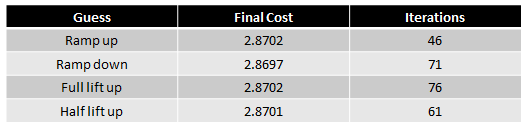
\includegraphics[width=1\textwidth]{Images/Convergence/ConvergeGuesses}
	\caption{KS statistics estimating the sensitivity of terminal altitude and range to the uncertain input variables.}
	\label{Table:ConvergeGuesses}
\end{table}

\section{Joint Optimization of Velocity-Varying Gains}s
A natural question is if DDP can be used to jointly optimize not only constant gains, but also velocity-varying gains as well. Given that constant gains are a special case of varying gains, the optimal solution with dynamic gains can do no worse than the constant gain solution, and is expected to perform better. In this section we present an example of optimized velocity-varying gains and discuss the issues. 
\begin{figure}[h!]
	\centering
	\includegraphics[width=1\textwidth]{Images/Trajectory/MCGridFailedGainOpt}
	\caption{Sample trajectories and 3$\sigma$ bounds estimated by MC and UT for a solution with jointly optimized, velocity-varying gains.}
	\label{Fig:GainOptTrajectory}
\end{figure}
\begin{figure}[h!]
	\centering
	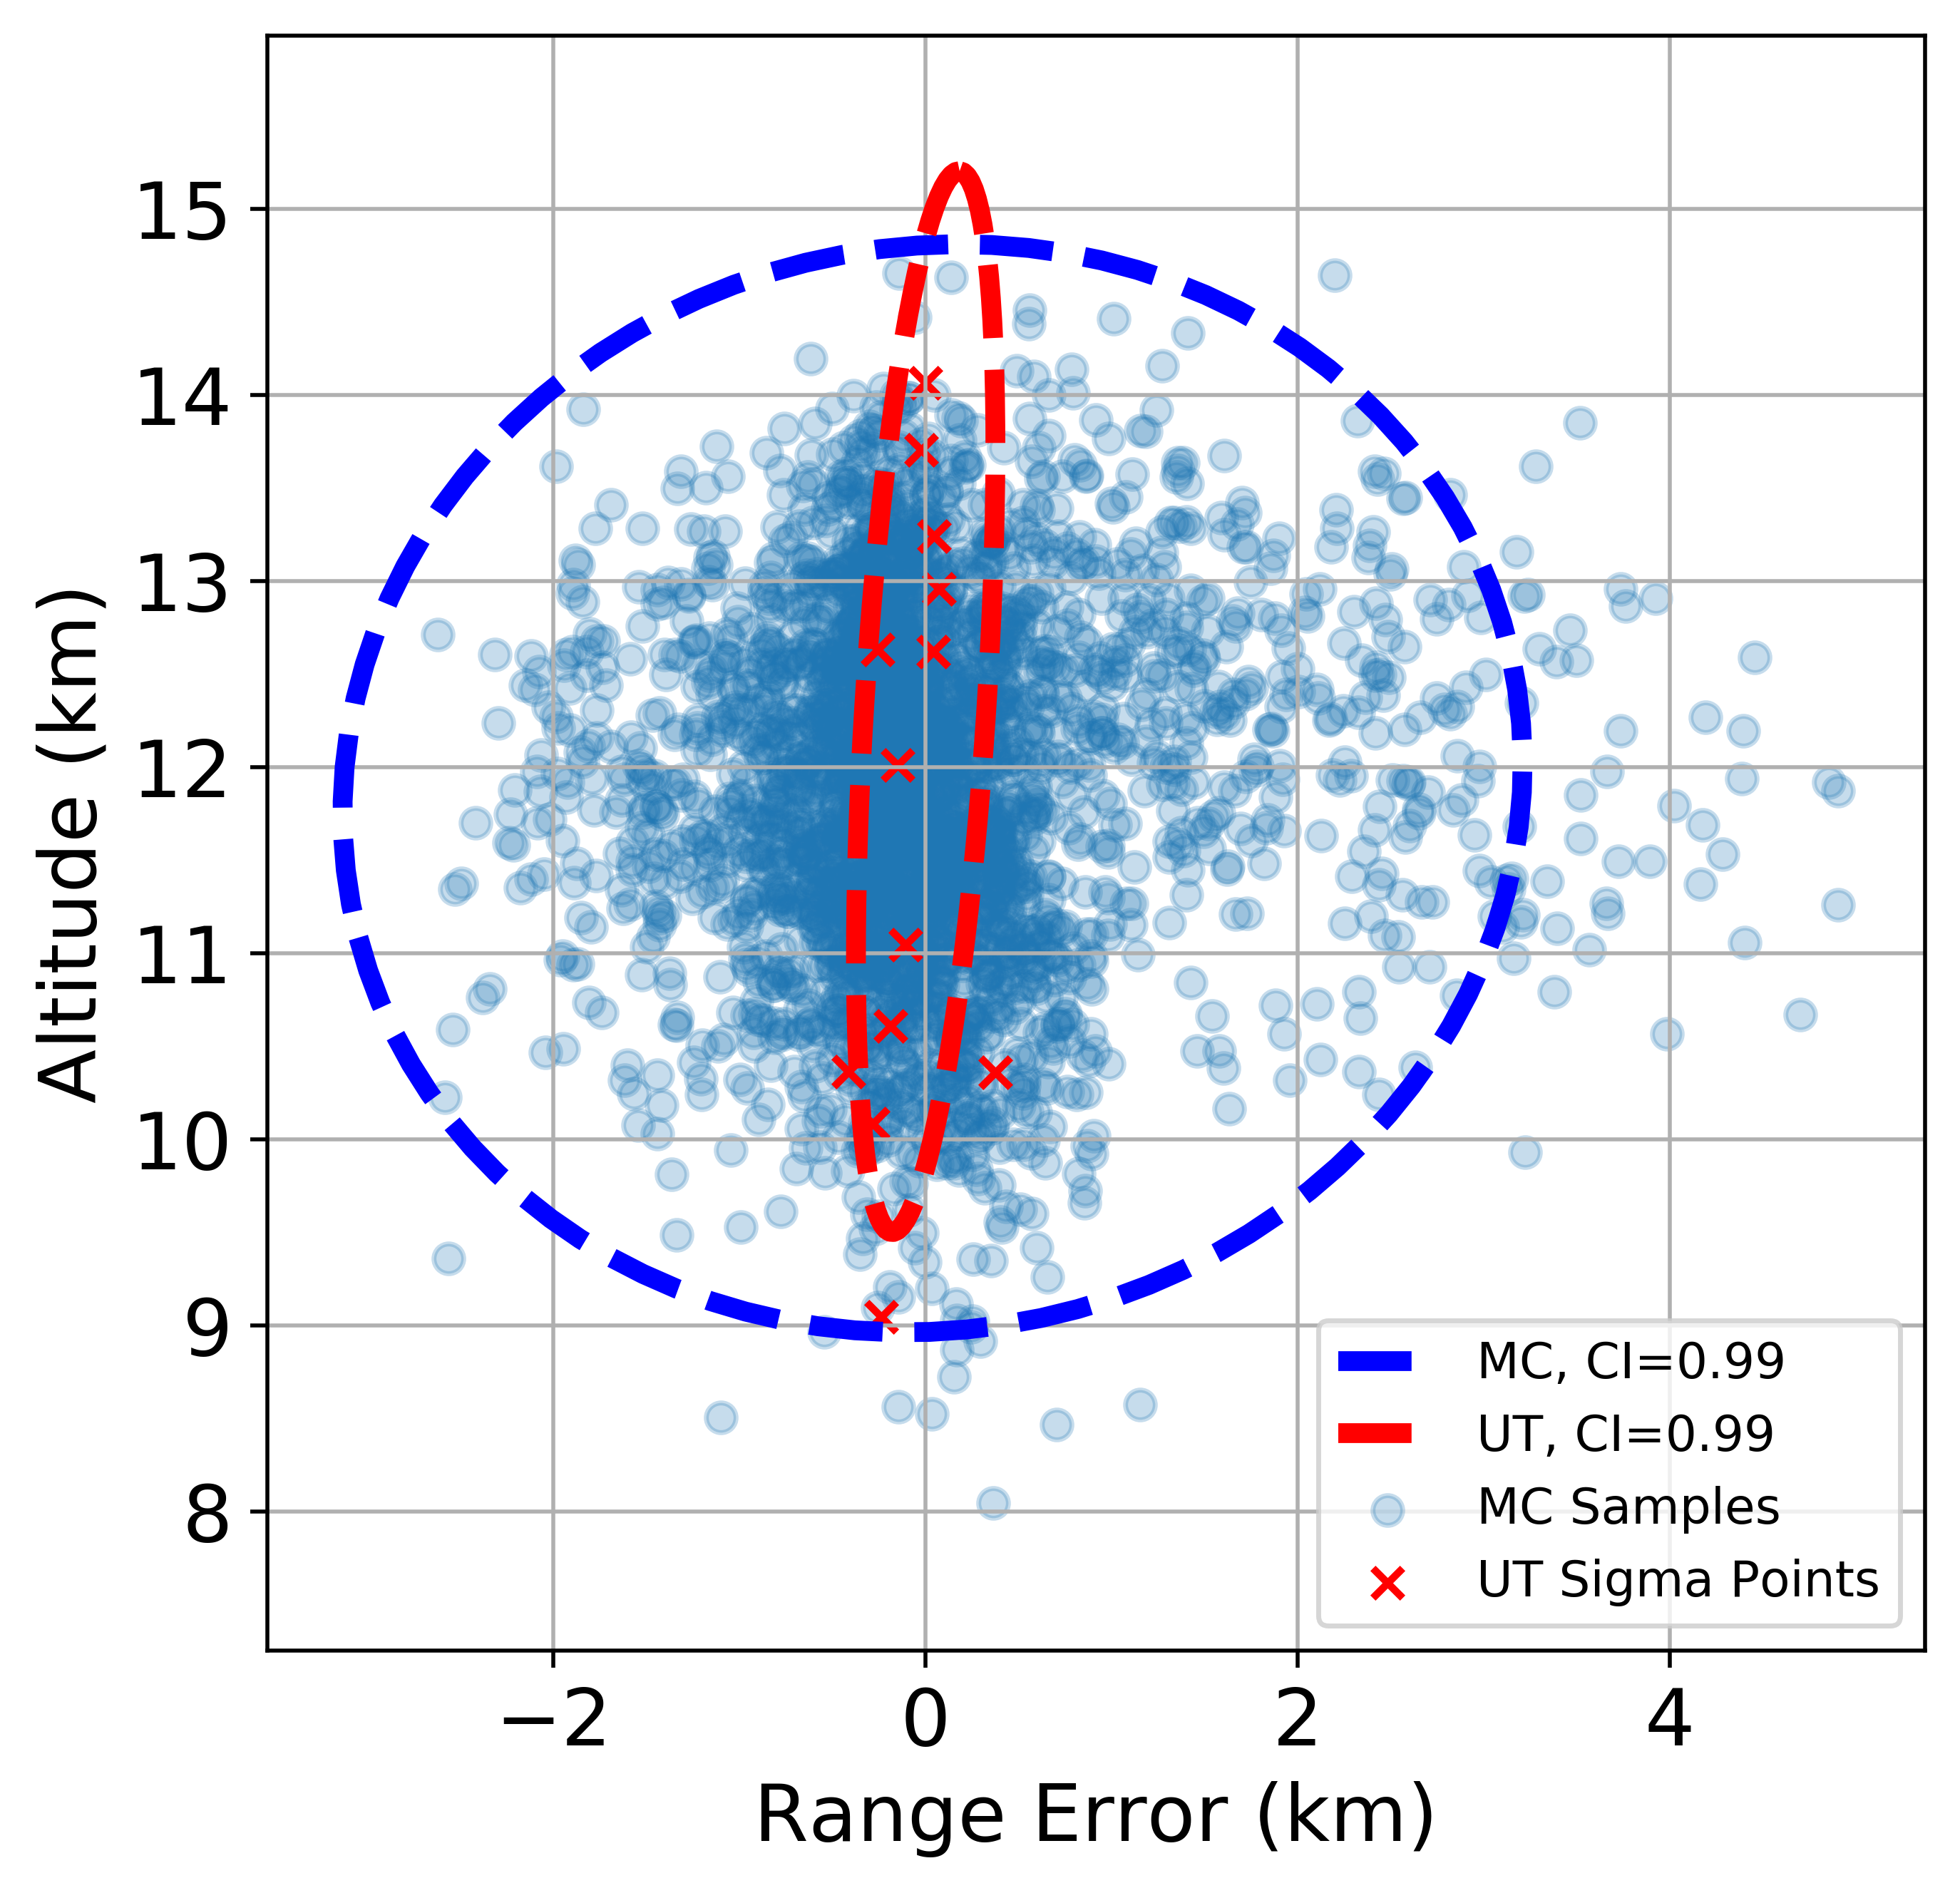
\includegraphics[width=1\textwidth]{Images/Trajectory/AltitudeRangeScatterFailedGainOpt}
	\caption{Terminal altitude and range performance for a solution with jointly optimized, velocity-varying gains.}
	\label{Fig:GainOptScatter}
\end{figure}
Figure~\ref{Fig:GainOptTrajectory} shows the MC results as well as the sigma points and estimated 3$\sigma$ bounds. It can be seen that the solution drives the sigma points to a narrow set of terminal ranges, and as such the UT estimates a small $\sigma_s=300$ m. However, the simulated performance in the Monte Carlo setting show the results are quite different from the UT. Figure~\ref{Fig:GainOptScatter} shows the terminal altitude and range flown. In this scenario, the UT is not accurately estimating the terminal statistics. This issue is reminiscent of the overfitting problem in machine learning, in which a solution that has a low value of the loss function over the sample points does not generalize well to samples not in the data set. The DDP solution is correctly guiding the sigma points together but fails to work well in other dispersed scenarios, such as those with a mix of the input uncertainties. It is evident the guidance does not perform as predicted and the size of the range error is not only larger than expected, but also larger than solutions with fixed gains. One apparent cause for the poor performance is the high gain nature of the solutions. Unless restricted to smaller magnitudes, the gains are, at times, quite large in magnitude, resulting in large control corrections and oscillatory commands that are not well-tracked due to the bank rate limit. Our experience with poor performance and poor agreement between the UT and MC statistics was part of the motivation to consider static feedback gains. In conclusion, while joint optimization of velocity-varying gains has the potential to improve performance compared to static gains, we were unable to do so, and additional work is needed to determine how to solve the issue discussed here. 

\section{Comparison to MSL and Mars 2020}
The exact conditions under which MSL and Mars 2020 assess their guidance are not presented in Refs.~\cite{MSL_EDL2,M2020_EDL}; thus a precise comparison cannot be made. Nevertheless several comparisons that may be drawn. MSL designers simulated the open-loop performance and found the 3$\sigma$ range error was approximately 40 km with a 3$\sigma$-low altitude of 6 km for a reference trajectory with 9 km nominal deployment altitude. Thus, the total effect of the stochastic parameters in their simulation is about 3 km 3$\sigma$ altitude loss and 40 km 3$\sigma$ range error. In performing the same exercise, we found that our 3$\sigma$ altitude loss was 2.5-3.1 km, and 3$\sigma$ range error was 59-66 km, each depending on the weights selected. With closed-loop guidance, and in the absence of onboard estimation errors, i.e., the case most similar to our assessment conditions, MSL reported a 3$\sigma$ range error at chute deploy of 7 km~\cite{MSL_EDL2}. In comparison, despite approximately 50\% larger open-loop range errors and comparable altitude losses, our approach achieves 3$\sigma$ range errors of 3.2 km and, like the ETPC, no additional altitude loss results from the closed-loop guidance. The 3$\sigma$-low altitude is 9.5 km, enabling targeting of site elevations above 0 km. Thus, while the results are not conclusive and additional testing is necessary, the proposed control law and design method appear promising in achieving high altitude while reducing range and altitude dispersions. 




%%% Local Variables: ***
%%% mode: latex ***
%%% TeX-master: "thesis.tex" ***
%%% End: ***
